%%% LATEX PRÄAMBEL %%%%%%%%%%%%%%%%%%%%%%%%%%%%%%%%%%%
\documentclass[11pt,a4paper]{article}
%\documentclass[11pt,a4paper,headsepline,notitlepage,cleardoubleempty,BCOR=20mm,twoside,DIV=12]{scrreprt}  
\usepackage[utf8]{inputenc}
\usepackage{color}
\usepackage{graphicx}
\usepackage[ngerman]{babel}
\usepackage{amsmath}
\usepackage{listings}
\usepackage{latexsym}
\usepackage{hyperref}
%\renewcommand{\baselinestretch}{1.50}\normalsize
\bibliographystyle{plain}
\bibdata{mybib}
\newtheorem{definition}{Definition}[section]
\newtheorem{function}{Funktion}[section]


%%% TITEL %%%%%%%%%%%%%%%%%%%%%%%%%%%%%%%%%%%%%%%%%%%%%
 \title{\small{Großer Beleg}\\\Large{Analyse von Ansätzen zur Beschleunigung von SAT-Lösern durch dedizierte Hardware-Komponenten}}
 \author{Erik Zenker}
 \date{22.07.2011}


%%% MAKROS %%%%%%%%%%%%%%%%%%%%%%%%%%%%%%%%%%%%%%%%%%%
\newcommand{\todo}[1]{\textcolor{red}{[TODO: #1]}}
\newcommand{\ru}[1]{\textcolor{black}{$\leadsto$ #1}}
\newcommand{\dec}[1]{\textcolor{black}{ #1^d}}
%\date{\dasdatum}

%%%%%%%%%%%%%%%%%%%%%%%%%%%%%%%%%%%%%%%%%%%%%%%%%%%%%%%
%%% DOKUMENT ANFANG %%%%%%%%%%%%%%%%%%%%%%%%%%%%%%%%%%%
\begin{document}
%%\maketitle
\begin{titlepage}
        \vspace*{\bigskipamount}
        \begin{center}
                \noindent
                \textbf{\LARGE{Großer Beleg}}\\[4ex]
                \noindent%
                \textbf{\huge{Analyse von Ansätzen zur Beschleunigung von SAT-Lösern durch dedizierte Hardware-Komponenten}}\\[10ex]
                \Large Erik Zenker\\[0.5ex]
	        \Large 14.08.2011\\[4ex]
                \LARGE Technische Universität Dresden\\
                \Large Fakultät Informatik\\
                \mbox{}\\
                Institut für Technische Informatik\\
                Professur für VLSI-Entwurfssysteme, Diagnostik und Architektur\\
                                 \mbox{}\\
                        Institut für Künstliche Intelligenz\\
                        Professur  für Knowledge Representation and Reasoning
        \end{center}
\begin{flushleft}
\vfill
Betreut von:

\textbf{Prof.\,Dr.-Ing.\,habil. Rainer G. Spallek}\\
\textbf{Prof.\,Dr.\,rer.\,nat. Steffen H\"olldobler (KI)}\\
\textbf{Dipl.-Inf. Thomas Preußer}\\
\textbf{Dipl.-Inf. Norbert Manthey (KI)}


\end{flushleft}
\end{titlepage}
\newpage
\mbox{} \thispagestyle{empty}
\newpage
Hier Aufgabenstellung einfügen
\newpage

\mbox{} \thispagestyle{empty}
\newpage
\tableofcontents 
\newpage
%%% EINLEITUNG %%%%%%%%%%%%%%%%%%%%%%%%%%%%%%%%%%%%%%%%
\section{Einleitung}

In der Informatik beschäftigt man sich mit einer Vielzahl von
kombinatorischen Problemen und wie diese effizient gelöst werden können.
Nicht jedes Problem ist gleich schwer bzw. leicht zu lösen, weshalb sie in
sogenannte Problemklassen eingeteilt werden.  Eine Klasse ist die Klasse der
nichtdeterministisch polynomiell vollständigen Probleme. Für NP-vollständige Probleme gibt es bisher
keine Möglichkeit, diese effizient zu lösen. Ein Durchprobieren von
allen Lösungsmöglichkeiten würde sehr viel Zeit in Anspruch nehmen und
wird deshalb nur bei kleiner Problemgröße durchgeführt. Deshalb
werden oft problemspezifische Heuristiken benutzt, wodurch trotz
exponentieller Komplexität durchaus gute Ergebnisse erzielt werden
können.  Auch das Erfüllbarkeitsproblem (engl. Satisfiability Testing SAT)
gehört zur Klasse der NP-vollständigen Probleme. Moderne SAT Solver
können SAT-Probleme mit mehreren millionen Variablen und Klauseln
lösen und werden beständig weiter entwickelt.\\ Die
Rechnerarchitekturen auf denen SAT-Solver ausgeführt werden ändern
sich unaufhaltsam in Richtung Many-Core-Architekturen. Bereits heutige
Serversysteme haben 12 unabhängige Rechenkerne \cite{amdopteron:2011} auf einem
Prozessorchip, und selbst einfache Desktopsysteme sind standardmäßig
mit 2 bis 4 Kernen ausgestattet.\\ Ein Nachteil von SAT-Solvern ist
bisher, dass ihr Algorithmus auf sequentielle Verarbeitung
optimiert ist, obwohl bereits mehrere parallele Einheiten zur Verfügung
stehen.  Deshalb müssen die Algorithmen angepasst werden, um
auch in Zukunft die vorhandenen Ressourcen effektiv ausnutzen zu können.\\ Man
kann noch einen Schritt weiter gehen. Statt der Auslagerung der Algorithmen
auf einige wenige Kerne, nutzt man die hohe Parallelität
von Field Programmable Gate Arrays (FPGAs).  Ein Ansatz ist es den
Inferenzmechanismus, welcher ca. 80 bis 90\% der Rechenleistung in
aktuellen SAT-Solver belegt, auf einen FPGA auszulagern und 
ihn hochparallel auszuführen.\\
%\todo{Hier noch ein bisschen mehr zu FPGAs einleiten}\\



%%% EINFÜHRUNG %%%%%%%%%%%%%%%%%%%%%%%%%%%%%%%%%%%%%%%%
\section{Einführung in das Thema}
Dieses Kapitel soll eine Einführung zum Thema SAT und 
FPGAs geben. In dem folgenden Unterkapitel
\ref{sec:intro_sat} wird auf das SAT-Problem, die 
zugrunde liegende Aussagenlogik und auf das in dieser
Arbeit benötigte Gruppieren von Formeln eingegangen.
Im Unterkapitel \ref{sec:sat_algo} wird der DPLL
Algorithmus als möglicher Lösungsansatz zum Lösen des SAT-Problems erläutert.
Grundlagen zum Thema FPGA werden im Unterkapitel 
\ref{sec:intro_fpga} vermittelt.

%%% EINFÜHRUNG SAT SOLVING %%%%%%%%%%%%%%%%%%%%%%%%%%%%
\subsection{Einführung in SAT}
\label{sec:intro_sat}
Im SAT-Problem oder auch Erfüllbarkeitsproblem
der Aussagenlogik wird die Frage gestellt ob eine
gegebene aussagenlogische Formel erfüllbar ist.
Das SAT-Problem is NP-vollständig, 
womit sich jedes Problem aus NP in
polynomieller Zeit auf SAT zurückführen lässt
\cite{cook:1971}. Somit gehört SAT auch zur Klasse NP
der Probleme, die in polynomieller Zeit mit einer
nichtdeterministischen Turingmaschine gelöst werden
können. Das Erfüllbarkeitsproblem ist nicht nur
komplexitätstheoretisch interessant, sondern auch
industrielle und wissenschaftliche Probleme können als
SAT-Problem formuliert werden. Um diese Probleme zu
lösen, wurden in den letzten Jahrzehnten effiziente 
Lösungsansätze entwickelt.\\
Bewährte Algorithmen zur Lösung von SAT sind DPLL, CDCL und SLS.
\begin{itemize}
\item
  \textbf{DPLL} \cite{davis:1962}\\
  Der Davis-Putnam-Logemann-Loveland (DPLL) Algorithmus
  ist Basis für eine Vielzahl von anderen
  SAT-Algorithmen und wird in dieser Arbeit verwendet.
\item
  \textbf{CDCL} \cite{mitchell:2004}\\
  Der Conflict Driven Clause Learning (CDCL) Algorithmus
  löst strukturierte Probleme besonders gut. Er baut
  auf DPLL auf und ist mithilfe vieler Verbesserungen
  heutiger Stand der Technik.
  
\item
  \textbf{SLS} \cite{hoos:2004}\\
  Mit Stochastik Local Search (SLS) Solvern kann nur
  die Erfüllbarkeit von Formeln gezeigt werden.
  Besonders zufällige Instanzen können mit dieser
  Art von Solvern effizient gelöst werden.
\end{itemize}


\subsubsection{Syntax der Aussagenlogik}
Das Alphabet $\Sigma$ der Aussagenlogik besteht aus 
einer (abzählbar) unendlichen Menge von 
aussagenlogischen Variablen ${\cal R} = \{p_1,p_1,\ ...\}$, 
einer Menge von Junktoren 
$\{\neg /1,\ \wedge /2,\ \vee /2,\ \rightarrow /2,\ \leftrightarrow /2\}$
und der Menge von Sonderzeichen $\{(,\ )\}$. Im Kontext
von SAT werden nur Formeln in konjunktiver Normalform
(KNF) betrachtet. Somit werden nur Begriffe in diesem 
Zusammenhang definiert. Da diese Definitionen Grundlagen
sind, wurden sie teilweise aus \cite{hoell:2009} übernommen.

  \begin{definition}
    Ein Atom ist eine aussagenlogische Variable.
   \end{definition}
  \begin{definition}
    Ein Literal ist eine aussagenlogische Variable oder
    eine negierte aussagenlogische Variable. Dabei wird
    eine aussagenlogische Variable auch positives Literal
    und eine negierte aussagenlogische Variable auch
    negatives Literal genannt.
  \end{definition}
  Im weiteren Verlauf werden
  Literale mit $l$ bezeichnet. Für konkrete Beispiele
  werden statt Buchstaben ganze Zahlen verwendet. Eine
  positive ganze Zahl entspricht einem positiven Literal,
  die gleiche ganze Zahl mit $-1$ multipliziert seiner
  Negation. Die Zahl 0 ist kein Literal, da sie weder
  negativ noch positiv ist. Ein Beispiel: 
  \begin{center}
    $l = 5$\\
    $\neg l = -5$
  \end{center}


  \begin{definition}
    Eine Klausel ist eine Disjunktion von Literalen.
  \end{definition}

  \begin{definition}
    Man nennt eine Klausel Unit oder Unit-Klausel, wenn
    sie nur aus einem Literal besteht. Dieses Literal wird 
    dann Unit-Literal genannt.
  \end{definition}
  \begin{definition}
    Eine Formel in KNF ist eine Konjunktion von Klauseln.
  \end{definition}
  \begin{function}
    Die Funktion $var(l)$, eines Literals $l$, gibt die
    ensprechende Variable von $l$ zurück.

  \end{function}
  \begin{function}
    Die Funktion $var(C)$ gibt die Menge von allen Variablen
    einer Klausel $C$ zurück.
  \end{function}
  \begin{function}
    Die Funktion $var(F)$ gibt die Menge von allen Variablen
    einer Formel $F$ zurück.
  \end{function}
  Klauseln werden ab jetzt immer mit dem Buchstaben $C$,
  Formeln mit $F$ und Literale mit $l$ dargestellt.
  Verschiedene Klauseln, Formeln bzw. Literale werden durch
  einen Index am Buchstaben unterschieden. Vereinfacht wird 
  eine Klausel statt 
  $((l_1 \vee l_2)\vee l_3)\vee ...\vee l_n)$
  in eckigen Klammern dargestellt 
  $[l_1, l_2, l_3,\ ..., l_n]$. Analog wird auch die 
  Schreibweise einer Formel in KNF vereinfacht. Statt 
  $((C_1 \wedge C_2)\wedge C_3)\wedge ...\wedge C_n)$ 
  schreibt man eine Formel wie folgt 
  $\langle C_1, C_2, C_3,\ ..., C_n \rangle$. Eine 
  Beispielformel könnte folgendermaßen aussehen.
  \begin{center}
    $F_{bsp} = \langle [1,3],[-2, 5, -6], [-1,-4,6], [-1,-2,-4,5], [-1,2]\rangle$
  \end{center}

  \subsubsection{Semantik der Aussagenlogik}
  Die Menge der Wahrheitswerte ${\cal W}$ ist die Menge
  $\{\top,\bot\}$. Dabei steht $\top$ für wahr und $\bot$
  für falsch. Man kann nun jeder aussagenlogischen Variable
  einen Wahrheitswert zuweisen. Verbindet man diese mit
  Junktoren zu Formeln, kann jeder Formel der Wert
  wahr oder falsch zuordnen werden, abhängig von den
  Wahrheitswerten der aussagenlogischen Variablen in der
  Formel.
  \begin{definition}
    Eine Interpretation ${\cal I}$ weist jeder
    aussagenlogischen Variable einer Formel einen
    Wahrheitswert zu.
    \begin{center}
    ${\cal I}: var(F)\rightarrow{\cal W}$
    \end{center}
  \end{definition}
  \begin{definition}
    Ein Literal ist erfüllt, wenn es eine
    aussagenlogische Variable ist, welche auf wahr
    abgebildet wird, oder eine negierte aussagenlogische
    Variable, welche auf falsch abgebildet wird.
  \end{definition}
  \begin{definition}
    Eine Klausel ist erfüllt, wenn mindestens ein Literal
    in der Klausel erfüllt ist. Die leere Klausel ist
    nach Definition unerfüllt.
  \end{definition}
  \begin{definition}
    Eine Formel ist erfüllt, wenn alle ihre Klauseln
    erfüllt sind. Eine leere Formel ist nach Definition
    immer erfüllt.
  \end{definition}
  \begin{definition}
    Eine partielle Interpretation ist eine
    Interpretation, welche nicht alle aussagenlogischen
    Variablen einer Formel $F$ auf einen Wahrheitswert
    abbildet.
  \end{definition}
  \begin{definition}
    Eine Interpretation, welche eine Formel $F$ erfüllt, 
    nennt man Modell von $F$.
  \end{definition}
  %% Eine partielle Interpretation kann auch als Menge von
  %% Literalen verstanden werden. Alle Literale in dieser Menge
  %% der partiellen Interpretation werden auf wahr und deren
  %% Negation auf falsch abgebildet. Undefiniert nennt man Variablen, wenn diese nicht
  %% in der partiellen Interpretation vorhanden sind.
  Eine partielle Interpretation wird als Liste von
  Literalen, welche auf wahr abgebildet werden,
  dargestellt. Sollte ein Literal oder seine Negation
  nicht in dieser Liste vorhanden sein, dann ist ihr Wahrheitswert
  undefiniert. Die Sortierung der partiellen
  Interpretation ist wichtig, da sie den aktuellen Pfad 
  im Suchbaum widerspiegelt. Ist zum Beispiel folgende
  partielle Interpretation gegeben $(l_1,l_2, ..., l_n)$,
  dann wurde das Literal $l_1$ im Suchprozess zuerst
  entschieden und  $l_n$ zuletzt. Eine partielle Interpretation,
  welche alle Variablen eine Formel enthält, nennt man total.\\
  \begin{definition}
    Ist $F$ eine Formel und $J$ eine partielle oder totale Interpretation, 
    dann ist $F|_J$ das Redukt bzw. das verbleibende
    Problem der Formel. 
  \end{definition}
  Das Redukt wird wie folgt gebildet:
    \begin{itemize}
      \item Alle Klauseln, welche mindestens ein erfülltes Literal
        aus $J$ enthalten, werden aus $F$ entfernt.
      \item Alle Literale, welche negiert in $J$ vorkommen,
        werden aus ihren Klauseln in $F$ entfernt.
    \end{itemize}
  Sei  nun die Formel $F_{bsp}$ aus dem
  vorherigen Abschnitt zusammen mit der partiellen
  Interpretation $J = (-1,-5)$ gegeben, dann ist
  $F_{bsp}|_J = \langle [3],[-2,-6]\rangle$
  das Redukt von $F_{bsp}$ unter $J$. Die Klausel 
  $[3] \in F_{bsp}|_J$ ist eine Unit-Klausel,
  mit dem Unit-Literal 3.


  \subsubsection{Gruppieren von Klauseln}
  Für das Lösen einer SAT-Instanz mit dem später
  vorgestellten Entwurf ist es nötig, die Formel in
  Gruppen von Klauseln zu unterteilen. Diese Gruppen
  haben die Eigenschaft, dass jede Variable maximal einmal
  vorkommt. Daraus folgt,
  das man maximal ein Literal pro Gruppe nach einem
  Inferenzprozess erhält. Es werden nun Begriffe
  definiert, die für die Gruppierung von Formeln 
  benötigt werden.
  \begin{definition}
    Eine Gruppe ist eine Menge von Klauseln.
    \begin{center}
      $G = \{C_1, ..., C_m\}$
    \end{center}
  \end{definition}

  \begin{function}
    Die Funktion $occ(v, G)$ berechnet die Anzahl der Vorkommen einer
    Variable $v$ in einer Gruppe $G$.
    \begin{center}
      $occ(v, G) = |\{C \mid C \in G, v \in var(C)\}|$
    \end{center}
  \end{function}

  \begin{definition}
    ${\cal G}^{(i)}$ ist eine Menge
    von Gruppen mit maximalem Variablen Vorkommen von $i$.
    \begin{center}
      ${\cal G}^{(i)} = \{G_1, ..., Gn\}$
    \end{center}
    Es gilt:
    \begin{itemize}
      \item
        ${\cal G}^{(i)}$ ist eine endliche Menge von 
        Gruppen $:\ |{\cal G}^{(i)}| \leq n$
      \item
        $\forall G \in {\cal G}^{(i)} : occ(v,G) \leq i$
    \end{itemize}
  \end{definition}

  \begin{function}
    Die Funktion $group: F \rightarrow {\cal G}^{(i)}$ ist
    eine bijektive Abbildung aus einer Menge von Klauseln (Formel) in die
    Menge von Gruppen. Es wird  jeder Klausel einer Formel 
    eindeutig eine Gruppe zugewiesen.

  \end{function}
  Die Anzahl von Vorkommen von Variablen in Gruppen wird
  im Weiteren auf $i = 1$ beschränkt. Damit ergeben sich
  die folgenden Eigenschaften.

  \begin{definition}
  Die Funktion $f: V \rightarrow {\cal N}_0$ ist die
  Knotenfärbung eines Graphen $G(V,E)$ ohne
  Mehrfachkanten. Man nennt $f$ gültig oder zulässig,
  falls zwei beliebige benachbarte Knoten nicht
  dieselbe Farbe besitzen. 
  \end{definition}
  Analog dazu ist auch 
  $group: {\cal C} \rightarrow {\cal G}^{(1)}$ eine
  Knotenfärbungsfunktion eines Graphen $G(F, Var)$,
  $Var = \{(C_x,C_y)\mid C_x, C_y \in F, \exists\ v \in var(F),\ v \in var(C_x), v \in var(C_y)\}$.
  Knoten des Graphen entprechen den Klausel von $F$,
  wobei zwei Knoten durch eine Kante verbunden 
  werden, wenn gleiche Variablen geteilt werden.
  Man nennt $group$ gültig oder zulässig,
  falls zwei beliebige benachbarte Knoten nicht
  dieselbe Gruppe besitzen. 
  Eine Formel $F_{group} = \langle C_1, C_2, C_3,C_4 \rangle =  \langle[1,2],[2,3],[3,4],[4,5]\rangle$
  entspricht dem Graphen in Abbildung \ref{formula}
  und kann mit $group: {\cal C} \rightarrow {\cal G}^{(1)}$
  auf verschiedene Weise in zwei verschiedene Farben
  (Gruppen) gefärbt werden (Abbildung \ref{formula_colored}).
  \begin{figure}[h]
    \centering
    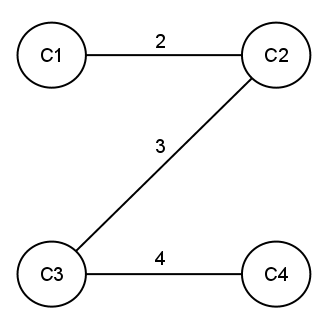
\includegraphics[width=0.25\textwidth]{abb/formula_graph.png}
    \caption{Graph zur Formel $F_{group}$}
    \label{formula}
  \end{figure}
   \begin{figure}[h]
    \centering
    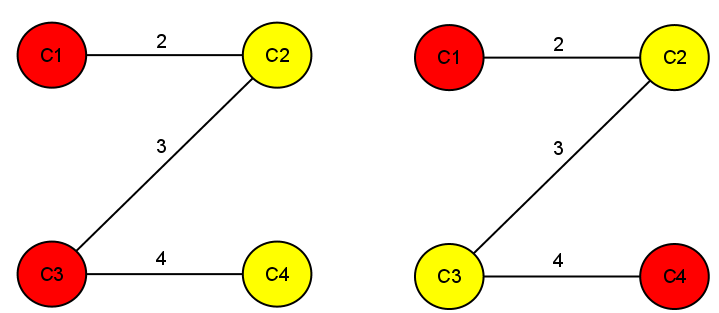
\includegraphics[width=0.5\textwidth]{abb/formula_graph_colored.png}
    \caption{Mögliche Färbung des Graphen zur Formel $F_{group}$}
    \label{formula_colored}
  \end{figure}
  Wenn ein Graph färbbar ist, gibt es eine kleinste
  Zahl $k$, sodass der Graph $k$-knoten-färbbar ist. 
  Diese Zahl wird die chromatische Zahl oder
  Knotenfärbungszahl des Graphen genannt und meist mit 
  $\chi(G)$ bezeichnet. Existiert für endlich viele
  Farben keine Färbung setzt man symbolisch $\chi(G)=\infty$.
  Die Bestimmung der chromatischen Zahl eines Graphen ist
  NP-schwer, das heißt, dass es aus Sicht der Komplexitätstheorie 
  vermutlich keinen Algorithmus gibt, der dieses Problem 
  effizient löst. Das bedeutet auch, dass die Bestimmung der
  kleinsten Anzahl n von Gruppen in ${\cal G}^{(1)}$ ein
  NP-schweres Problem ist.\\
  Für größere SAT Probleme, ist eine 
  intelligente Heuristiken nötig um ein schnelles Gruppieren
  zu gewährleisten.

%%% Algorithmen zum lösen des SAT Problems %%%%%%%%%%%%
\subsection{Lösen des SAT-Problems}
\label{sec:sat_algo}
Dieses Unterkapitel beschreibt den bereits seit 1962
existierenden DPLL-Algorithmus \cite{davis:1960}.
Ursprünglich wurde dieser 
Algorithmus eingesetzt, um Unerfüllbarkeit zu zeigen. 
In dieser Arbeit wird eine Version vorgestellt, welche die
Lösbarkeit von Formeln zeigt.\\
%\todo{bessere Einleitung}\\

\subsubsection{Suchbäume}
Ein Suchbaum ist ein binärer Baum. Jeder Knoten $t$ hat
genau zwei Nachfolgeknoten $t_1$ und $t_2$. Kanten zwischen zwei Knoten werden
mit Literalen beschriftet. Ist eine Kante $t \rightarrow t_1$ zu einem
Kindsknoten mit $l$ beschriftet, dann muss die Kante $t \rightarrow t_2$
zu dem anderen Kindsknoten mit $\neg l$ beschriftet sein. Desweiteren
darf die Variable des Literals, welche zur Beschriftung einer Kante benutzt
wurde, nicht bereits auf dem Pfad vom Wurzelknoten zum Knoten $t$ benutzt
worden sein.
 \begin{figure}[h]
    \centering
    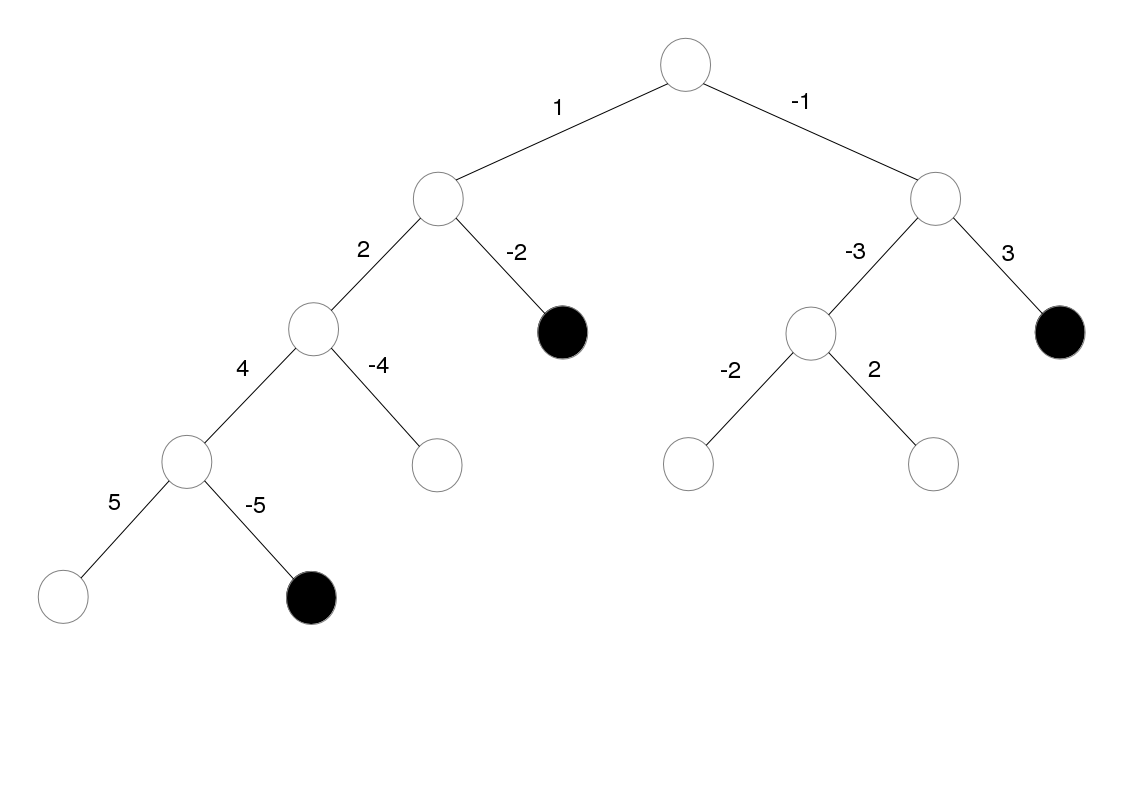
\includegraphics[width=\textwidth]{abb/suchbaum.png}
    \caption{Beispiel für einen Suchbaum}
    \label{suchbaum}
  \end{figure}
Der Pfad von einem Knoten $t$ zum Wurzelknoten entspricht der partiellen
Interpretation, welche alle Literale auf diesem Pfad enthält. Die Suche
kann auf einem Pfad beendet werden, wenn die partielle Interpretation 
des Pfades jedes Literal einer Klausel $C$ der Formel $F$ nicht erfüllt. Da bereits alle
Literale, welche $C$ enthält, auf dem Pfad vorkommen und $C$ weder
undefiniert noch erfüllte Literale enthält, kann man $F$ nicht erfüllen,
indem man weitere Literale zum aktuellen Suchpfad hinzufügt. Deshalb
kann dieser Pfad geschlossen werden. Sollte ein Pfad alle
Variablen von $F$ enthalten und alle Klauseln erfüllen,
dann ist die entsprechende Interpretation ein Modell
von $F$.\\
Ein Suchbaum wird also solange durch Hinzufügen
von neuen Kindsknoten erweitert, bis ein Pfad gefunden wurde, welcher
alle Variablen enthält, oder alle Pfade mit einer
unerfüllten Klausel enden. Wurde ein Modell gefunden, dann ist
die Formel erfüllbar.\\
Abbildung \ref{suchbaum} zeigt einen nicht vollständig expandierten
Suchbaum der Beispielformel $F_{bsp}$. Schwarze Knoten im Baum 
stellen nicht erfüllende Pfade dar.

\subsubsection{Davis Putnam Logemann Loveland Algorithmus}
Der Davis Putnam Logemann Loveland (DPLL) Algorithmus
erzeugt mithilfe von speziellen Regeln einen Suchbaum.
In Abbildung \ref{dpll} ist der Algorithmus als Flussdiagramm
angegeben. 
 \begin{figure}[h!]
    \centering
    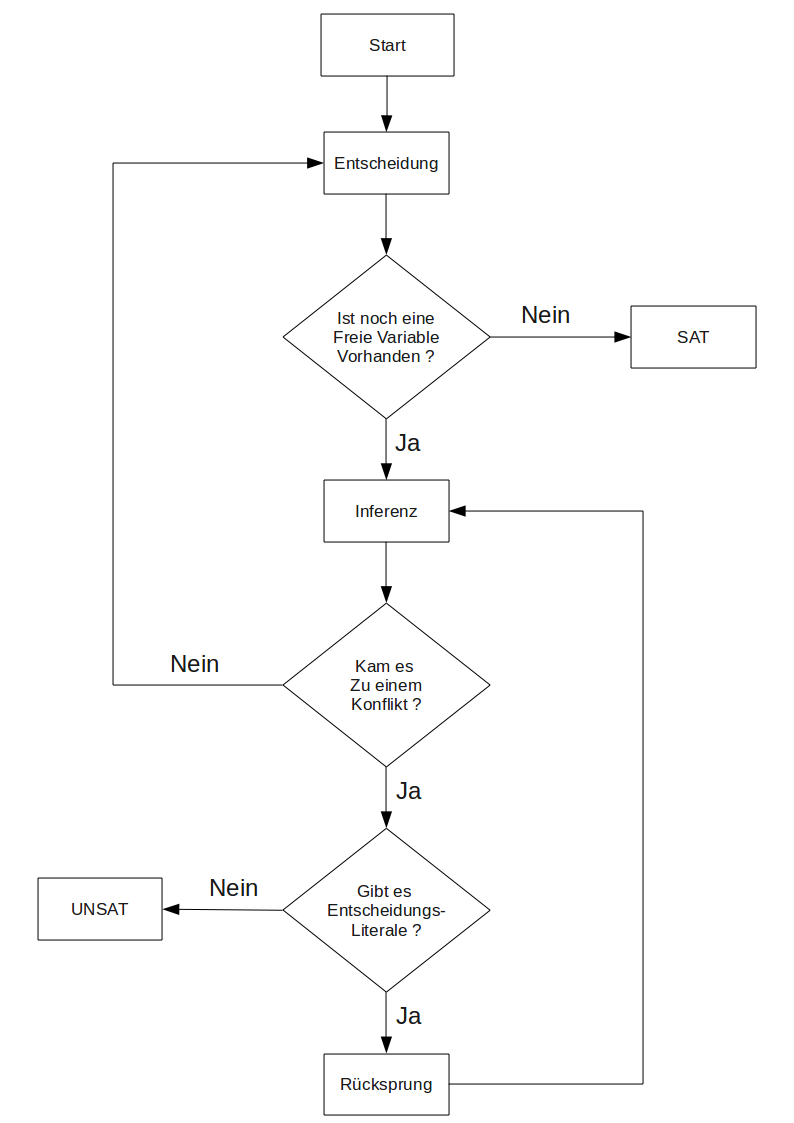
\includegraphics[width=0.75\textwidth]{abb/dpll.png}
    \caption{Flussdiagramm des DPLL-Algorithmus}
    \label{dpll}
  \end{figure}
Unit Literale in der Ausgangsformel
können der partiellen Interpretation hinzugefügt werden.
Es wird damit begonnen, sich für eine freie Variable
zu entscheiden, das heißt eine Variable oder die negierte
Variable, welche noch nicht in der partiellen Interpretation
enthalten ist, wird auf wahr abgebildet. Das Literal wird 
Entscheidungsliteral genannt. Sollte keine freie
Variable mehr vorhanden sein, dann beendet man den Prozess
mit SAT. Wenn sich für eine Variable entschieden wurde, dann 
wird mit der Inferenz der Formel begonnen. Im Inferenzprozess 
sucht man nach Unit-Klauseln im Redukt der Formel. Findet
man unter der aktuellen partiellen Interpretation
eine solche Unit, wird das Literal dieser Klausel
der partiellen Interpretation hinzugefügt und der Inferenzprozess
beginnt erneut. Dies geht solange, bis das Redukt der 
Formel keine Units mehr enthält. Kommt es nicht zum
Konflikt entscheidet man sich für die nächste Variable.
Sollte das Redukt jedoch eine leere Klausel enthalten, 
bedeutet dies, dass alle Literale der Klausel nicht
erfüllt sind und somit die Klausel bzw. die Formel nicht 
erfüllt ist (Konflikt). Wenn sich kein Entscheidungsliteral
in der partiellen Interpretation befindet, dann wird
der Prozess mit ``nicht erfüllbar'' (UNSAT) beendet. Ist mindestens ein
Entscheidungsliteral vorhanden, dann werden alle
Literale bis zu diesem Literal von der partiellen 
Interpretation entfernt und das negierte Entscheidungsliteral
wieder hinzugefügt. Dieses negierte Literal ist selbst
kein Entscheidungsliteral mehr. Nach dem sogenannten Rücksprung
wird wieder eine Inferenz 
der Formel angestoßen.
 \begin{figure}[h!]
    \centering
    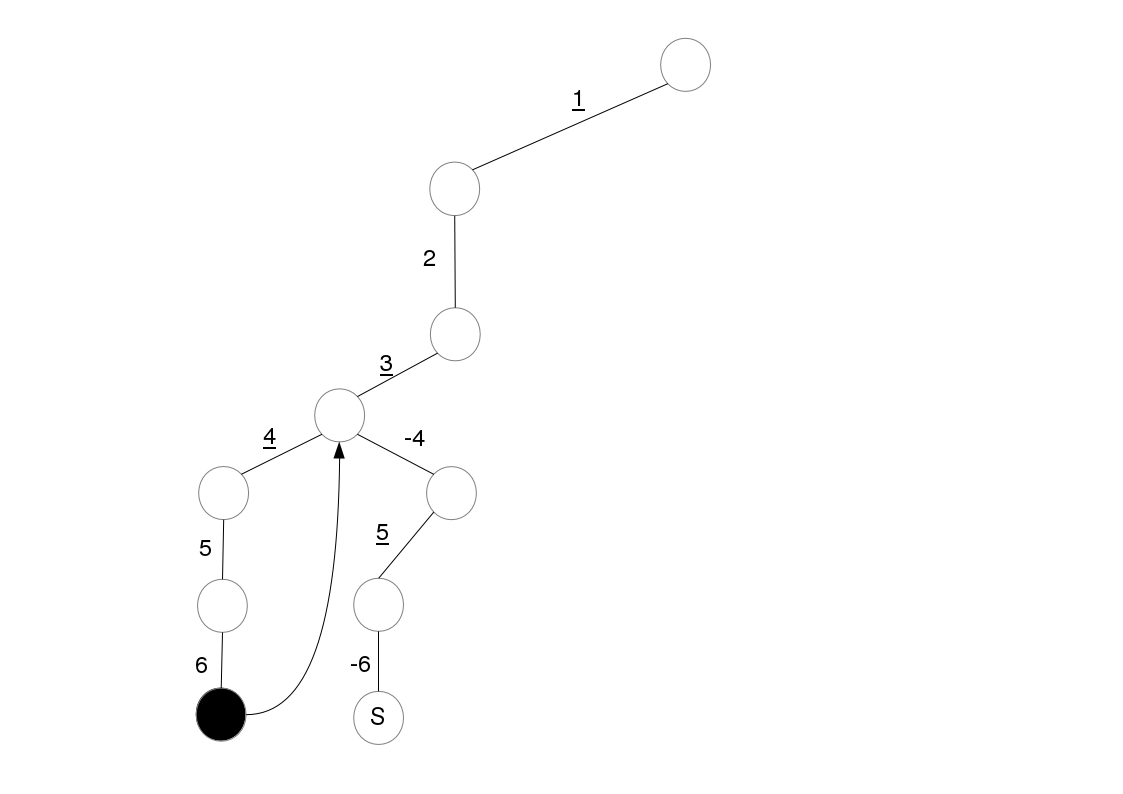
\includegraphics[width=\textwidth]{abb/dpll-suchbaum.png}
    \caption{DPLL-Suchbaum}
    \label{dpll-suchbaum}
  \end{figure}
Wendet man nun den vorgestellten DPLL-Algorithmus aus Abbildung
\ref{dpll} auf $F_{bsp}$ an, entsteht der Suchbaum in Abbildung
\ref{dpll-suchbaum}. Die Entscheidungsheuristik entscheidet 
sich in diesem Beispiel immer für die kleinste freie Variable.
Dieser Suchbaum weißt die Besonderheit auf,
dass manche Knoten nur einen Kindsknoten besitzen. Dies folgt
aus der Inferenz der Formel, da man gezwungen ist
Literalen einen gewissen Wahrheitswert zuzuweisen, um die Klausel zu
erfüllen. Literale welche im Suchbaum unterstrichen sind, 
sind Entscheidungsliterale. Werden Pfade mit S beschriftet, 
dann ist die partielle Interpretation dieses Pfades ein 
Modell der Formel.


\subsection{Einführung in FPGAs}
\label{sec:intro_fpga}
Ein Field Programmable Gate Array (FPGA) besteht 
hauptsächlich aus Speichern (FlipFlops \cite{scarbata:2001}) 
und davor geschaltenen Logikelementen,
welche in einer Matrix angeordnet sind.
Diese Logikelmente sind LUTs
(Lookup Tables), die über eine Programmierung die
gewünschte Funktion realisieren. Abbildung \ref{fpga} 
skizziert den Aufbau eines FPGA-Schaltkreises.
\begin{figure}[h]
  \centering
  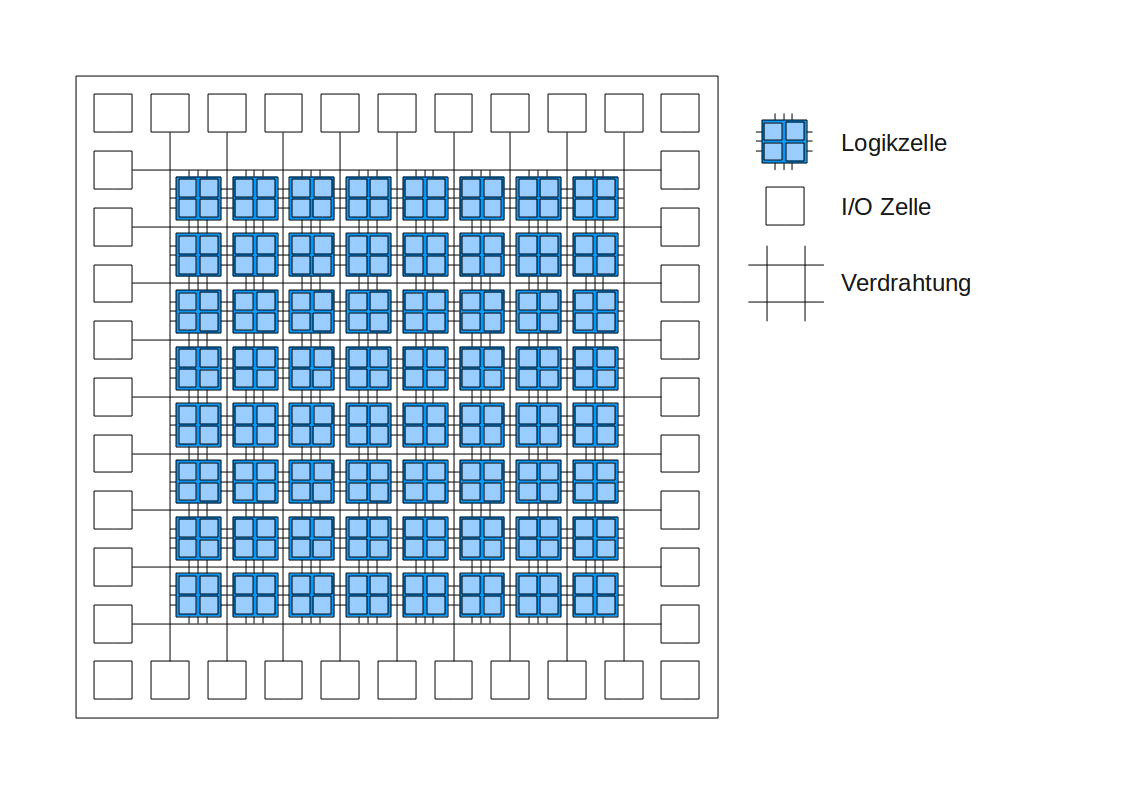
\includegraphics[width=\textwidth]{abb/fpga.png}
  \caption{FPGA-Skizze}
  \label{fpga}
\end{figure}
Eine LUT mit k Eingängen kann eine beliebige k-stellige
Binärfunktion realisieren. Die Anzahl von
Eingangssignalen pro LUT ist vom FPGA abhängig
und liegt meist zwischen 4 und 6 Eingangssignalen.
LUTs mit mehr Eingängen werden in der Regel nicht
gefertigt, da diese eine potenziell schlechtere
Auslastung aufweisen. Für Funktionen, die mehr
Eingänge erfordern als eine einzige LUT bietet,
werden mehrere LUTs direkt miteinander verschaltet.
Die Programmierung der gewünschten Funktion erfolgt
durch die Hinterlegung der definierenden Wahrheitstabelle
in den Speicher-Zellen der LUT, die Funktionsberechnung 
durch das Auslesen der durch die Eingänge bestimmten
Speicheradresse. Die Speicher sind in den meisten
FPGAs durch SRAM-Speicherzellen realisiert, welche
beim Konfigurationsprozess geladen werden.
Das Laden dieser Konfigurationsdaten bzw.
Verknüpfungsregeln geschieht dabei in der Regel aus
einem speziellen Flash-ROM Baustein heraus. Man kann den
FPGA über entsprechende Schnittstellen (JTAG \cite{ieeejtag:1990}),
konfigurieren um dessen Funktion zu implementieren.
Im Allgemeinen sind LUTs nur lesbar, es gibt jedoch auch Erweiterungen,
mit denen die Speicher der LUTs ebenfalls beschrieben
werden können.
Diese Technologie heißt Distributed RAM.
Abbildung \ref{lut} zeigt eine LUT mit
4 Eingängen und ein dahinter geschaltener FlipFlop.
\begin{figure}[h]
  \centering
  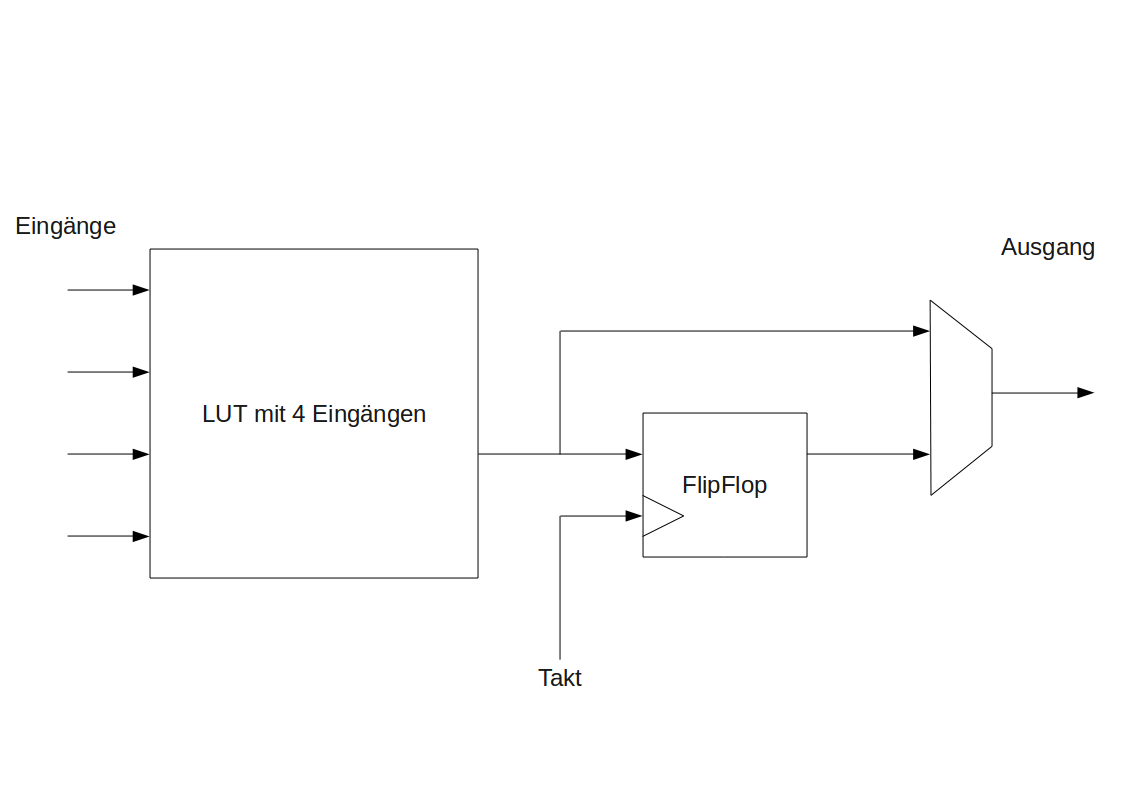
\includegraphics[width=\textwidth]{abb/logikzelle.png}
  \caption{Einfache Logikzelle}
  \label{lut}
\end{figure}
Die FlipFlops dienen dazu, Signalwerte
zwischenzuspeichern, um sie im nächsten Takt
weiterverarbeiten zu können. Meist wird
jeder LUT genau ein FlipFlop zugeordnet.
Eine Kombination von FlipFlop und Logikelement
wird zu einer Logikzelle (CLB) zusammengefasst.
Es können auch mehrere LUTs / FlipFlops in einer
Logikzelle zusammengefasst werden, dies variiert von
Hersteller zu Hersteller. Aktuelle FPGAs bestehen aus
mehreren zehntausend Logikzellen. Alle LUTs arbeiten
unabhängig voneinander und somit parallel.\\
Neben den Logikzellen beinhalten FPGAs darüberhinaus
komplexe Verdrahtungsnetzwerke, um Logikzellen auf
gewünschte Weise zu verbinden. Desweiteren stehen
meist noch zusätzliche Funktionsblöcke 
(auch Hard Macros genannt) zur Verfügung, welche bereits
eine vordefinierte Funktion erfüllen. Dies sind zum Beispiel
Multiplizierer, Taktgeneratoren \\ oder Block-RAMs \cite{xilinxbram:2005}.\\
Block-RAMs sind verteilte Speicher auf dem FPGA und lassen sich
auf vielfältige Weise ansprechen. So können 
damit Single- oder Dualport-RAMs mit variabler Bitbreite
erzeugt werden. Üblich sind mehrere kleinere 
Dualport-Block-RAMs von 18Kbit (Xilinx FPGAs).\\ 
Der FPGA-Chip wird von
einer Vielzahl von I/O Blöcken umrandet. I/O Zellen dienen der
Kommunikation mit der Außenwelt. Über I/O Blöcke werden
die Anschlüsse des FPGAs mit der Schaltmatrix verbunden.
Auch diese I/O Blöcke können an die jeweilige Anwendung
angepasst werden, z. B. kann die Ausgangsspannung an
den jeweiligen Standard angepasst \\werden (TTL/CMOS usw.).\\
Programmiert bzw. konfiguriert wird der FPGA mittels
einer Hardwarebeschreibungssprache (HDL) wie VHDL oder Verilog. 
Die Speicherbelegung der Logikzellen übernimmt dabei ein
Synthesewerkzeug, welches aus dem HDL-Quelltext die
Konfiguration synthetisiert.




%%% FPGA SAT %%%%%%%%%%%%%%%%%%%%%%%%%%%%%%%%%%%%%%%%%%
\section{FPGA-SAT}
Es hat sich gezeigt, dass sich mithilfe von FPGAs und angepassten 
Algorithmen Probleme wesentlich effizienter lösen lassen
als mit Universal-Prozessoren \cite{preusser:2009}\cite{dietrich:2009}. 
So kann auch das SAT-Problem und dessen\\Lösungsalgorithmen 
auf die Verarbeitung in FPGAs angepasst werden.
In diesem Kapitel wird auf die bisherige Arbeit im Bereich
Hardware-SAT-Solver eingegangen und zwei Entwürfe, welche
am vielsversprechendsten sind, kurz erläutert. 
Eine Zusammenfassung der genutzten 
Techniken bis 2004 wird gegeben von
Skliarova \cite{ferrari:2004} und
bietet einen Überblick zum Thema FPGA-SAT.

\subsection{Kategorisierung von Hardware-SAT-Solvern}
Skilarova \cite{ferrari:2004} unterschiedet, auf welche Art
und Weise man SAT-Probleme mithilfe von Hardware löst. 
Diese Kategorisierung von Hardware-SAT-Solvern wird auch in dieser Arbeit
aufgegriffen. Unterschieden werden typische SAT-Algorithmen wie DPLL, CDCL bzw. SLS, 
aber auch verwendete Entscheidungsheuristiken bzw. andere Techniken moderner
Software-SAT-Solver.\\
Desweiteren unterscheidet man das genutzte Programiermodell.
Für jede SAT-Instanz kann ein neuer Schaltkreis 
generiert werden, dann spricht man vom instanzspezifischen Programmiermodell 
oder man entwirft einen Schaltkreis, welcher 
synthetisiert verschiedene Instanzen 
lösen kann, dann spricht man vom aplikationsspezifischen Modell.\\
Das dritte Unterscheidungsmerkmal ist das Ausführungsmodell. 
Man kann den kompletten SAT-Solver in Hardware auf einem FPGA 
realisieren,dann ist es eine reine Hardware Lösung, oder man lagert
Teilkomponenten in Hardware aus, 
dann wird von einer Hardware / Software-Hybrid-Lösung gesprochen.\\

\subsection{Vorhandene Hardware-SAT-Solver}
Erste reine Hardware-Lösungen im Zeitraum von 1996 bis 2004
waren meist instanzspezifische Solver und für Probleme bis 
100 Variablen ausgelegt. Instanzspezifische Entwürfe benötigen 
bei neuen Instanzen Zeit um eine Synthese durchzuführen, wobei 
das eigentliche Lösen des Problems dann sehr schnell geschieht.
Diese Hardware-SAT-Solver wurden entworfen bevor
moderne SAT-Solver \cite{manthey:2010} ihren Siegeszug in der
Software-Welt antraten, sodass es eine Zeit lang keine weiteren Veröffentlichungen 
gegeben hat und ein Performancevergleich nicht möglich war.\\
Ab 2008 findet man erste Arbeiten, welche bei der Problemkomplexität 
mit modernen Software-Solver mithalten können. 
Eine Arbeit von John D. Davis et al. \cite{davis:2008} 
beschreibt einen applikationspeziafischen Hybrid-Entwurf auf CDCL-Basis.
Ein Host-PC übernimmt die Berechnung von Entscheidungsvariablen und die Analyse 
von Konflikten. Auf den FPGA wurde die Inferenz-Komponente ausgelagert. 
Davis Solver kann Probleme mit bis zu 64\,k Variablen und 64\,k Klauseln lösen.\\
Eine weitere Arbeit von Leopold Haller et al. \cite{haller:2010} 
beschreibt auch einen applikationsspezifischen Entwurf, jedoch wurde 
kein Host-PC für verschiedene Berechnungen benutzt. Dieser   
Entwurf ist in reiner Hardware realisiert. Durch die Nutzung von großen 
DRAM-Speichern können Probleme von bis zu 1\,M Variablen und 70\,M 
Klauseln berechnet werden. Leider fehlen in dieser Arbeit Resultate.\\
Nach ausführlichem Literaturstudium stellt man fest,
dass es zwar FPGA-SAT-Implementierungen gibt und diese
zu einer Beschleunigung der Algorithmen führen, jedoch fehlt
der Vergleich zu modernen Software-SAT-Solvern.\\
%\todo{man könnte hier noch ausführlicher schreiben, zumindest bis
%die Seite voll ist}


%%% SYSTEMÜBERBLICK %%%%%%%%%%%%%%%%%%%%%%%%%%%%%%%%%%%
\section{Systemüberblick}
Der in dieser Belegarbeit entstandene Entwurf basiert auf den 
Ideen von John D. Davis et al. \cite{davis:2008}. Es handelt sich um einen
applikationspezifischen Hybrid-Solver. Jedoch weicht er an einigen 
Stellen von dem ursprünglichen Design ab. So können wesentlich weniger
Variablen bearbeitet werden, es werden keine neuen Klauseln gelernt,
die Inferenz arbeitet mit Arbitern und der zugrunde liegende Suchalgorithmus ist DPLL statt CDCL. \\
Die Anzahl von Variablen, welche bearbeitet werden können,
ist geringer, da nur die auf dem FPGA befindlichen Block-RAMs genutzt werden.
Im ursprünglichen Entwurf wird zusätzlich noch ein DRAM-Speicher genutzt.
Auf die Nutzung von CDCL wurde verzichtet, weil der Algorithmus keinen Einfluss
auf den Inferenzprozess hat, sondern den Suchbaum anders als der DPLL-Algorithmus erzeugt.\\
In diesem Abschnitt werden die einzelnen Komponenten bzw. Module
des Entwurfs erläutert. In der folgenden Abbildung \ref{system} ist der Entwurf 
vereinfacht skizziert, um einen Überblick über das Gesamtsystem zu geben.
\begin{figure}[h]
  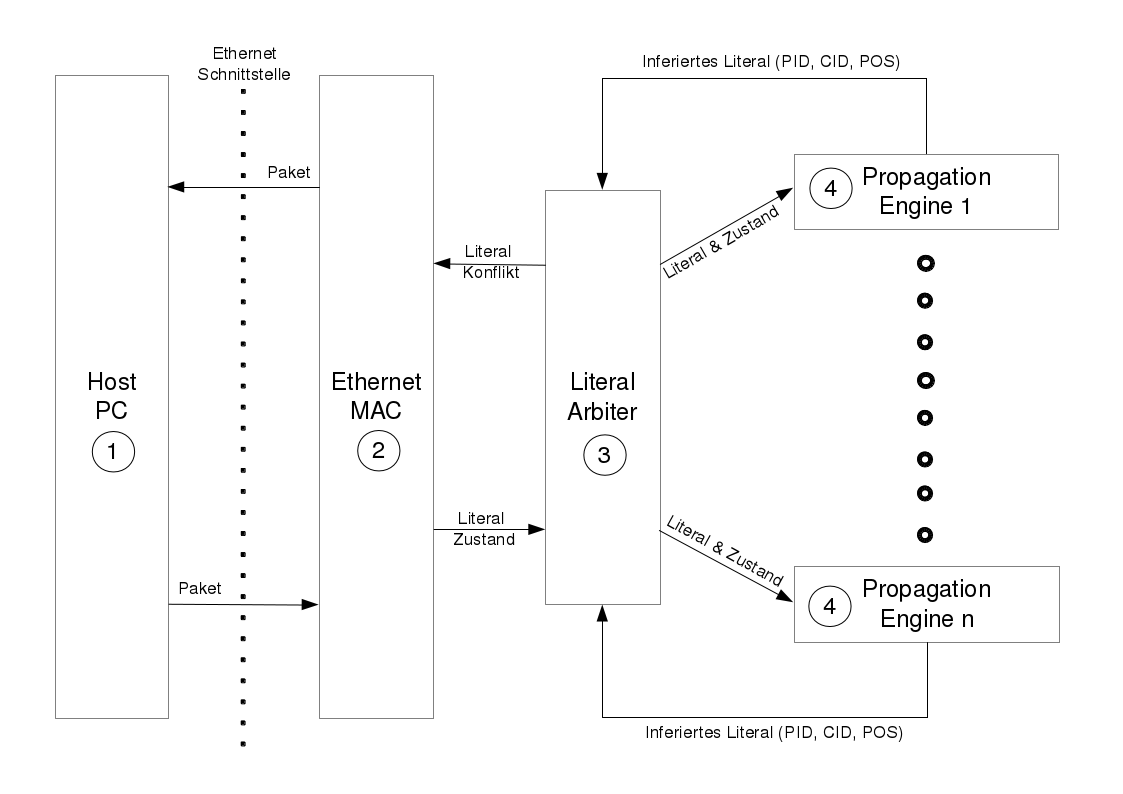
\includegraphics[width=\textwidth]{abb/system.png}
  \caption{Systemüberblick}
  \label{system}
\end{figure}
Ziel des Systems ist es, Entscheidungsliterale des Host-PCs so lange zu propagieren,
bis keine weiteren Literale propagiert werden können oder es zu einem 
Konflikt kommt. Im Konfliktfall muss vom Host-PC ein Rücksprung auf der
partiellen Interpretation durchgeführt und dem FPGA mitgeteilt werden.
Andernfalls muss der FPGA mit neuen Entscheidungsliteralen versorgt werden.\\
Es können mit diesem Entwurf Formeln mit bis zu 256 Variablen und 
4096 Klauseln gelöst werden. Eine Klausel darf dabei nicht mehr
als 9 Literale beinhalten. 
Die Variablen- und Klauselanzahl wird dabei durch die verfügbaren 
Block-RAM-Speicherressourcen der Literal-Übersetzungstabelle 
im Literal-Arbiter begrenzt.

\begin{enumerate}
\item Host-PC \newline
  Der Host-PC gruppiert die zu lösende Formel, übernimmt die Berechnung 
  von Entscheidungsliteralen und bestimmt den Rücksprungpunkt bei Konflikten.
  Er ist über eine Ethernet Schnittstelle 
  mit dem FPGA verbunden und kommuniziert mit diesem über Ethernet-Pakete.
  Mithilfe dieser Pakete steuert der Host-PC die Funktion des FPGAs.
\item Ethernet-MAC (Media Acces Control) \cite{xilinxether:2011}\newline
  Der Ethernet-MAC nimmt die Pakete des Host-PCs entgegen, verarbeitet 
  diese und gibt die enthaltenen Daten an den Literal-Arbiter weiter.
  Je nach Markierung von Ethernet-Paketen wird der FPGA in verschiedene Zustände versetzt, 
  wobei dadurch Eingabedaten anders verarbeitet werden.
  Außerdem werden durch den Ethernet-MAC Pakete erstellt,
  welche er an den Host-PC
  sendet. Diese Pakete enthalten Information über den
  aktuellen Suchprozess (inferierte Literale, Konfliktinformationen).
\item Literal-Arbiter \newline
  Der Literal Arbiter entscheidet welche Literale als nächstes propagiert 
  werden sollen. Außerdem führt er bei inferierten Literalen eine 
  Literal-Übersetzung durch. Die Übersetzung ist notwendig, da man Literale
  in den Propagation-Engines nicht durch eine ganze Zahl, sondern
  durch ein Tupel aus Gruppenindex, Klauselindex und
  Position des Literals in der Klausel darstellt.
  Sollte es zu einem Konflikt kommen oder ein Literal
  doppelt propagiert werden,  
  wird auch dies im Literal-Arbiter erkannt. Konfliktinformationen
  und inferierte Literale werden an den Ethernet-MAC weitergeleitet.
\item Propagation-Engine \newline
  Die Propagation Engine besteht aus zwei Hauptkomponenten. 
  Das ist zum einen das Literal-Lookup-Modul, welches bei gegebener 
  Variable die zugehörige Klausel, Position und Polarität 
  bestimmt und zum anderen das Status-Tabellen-Modul, welches 
  je nach Zustand eine Inferenz bzw. einen Rücksprung für eine Klausel durchführt.
  Dieses Modul wird mehrfach generiert und entspricht einer 
  Gruppe $G_k \in {\cal G}^{(1)}$.
\end{enumerate}
In Abbildung \ref{modi} werden die Abhängigkeiten zwischen
den Zuständen des Solvers dargestellt.
Der FPGA beginnt damit, im Wartezustand auf Eingaben
des Host-PCs zu warten. Er teilt dabei dem Host-PC über
ein Ethernet-Paket mit, dass er gerade keine Aufgaben hat.
Überlicherweise wird der FPGA zuerst initialisiert, indem die zu lösende
Formel in den Speicher des FPGAs geladen wird. Die Inferenz beginnt
nun durch ein erstes Entscheidungsliteral in einem Entscheidungpaket.
Sollte es während des Inferenzzustandes zum Konflikt kommen, dann wartet
der FPGA im Konfliktzustand solange ab, bis ein Rücksprungpaket
vom Host-PC empfangen wird. Ist der Rücksprung beendet, kehrt
der FPGA in den Wartezustand zurück.
\begin{figure}[h]
  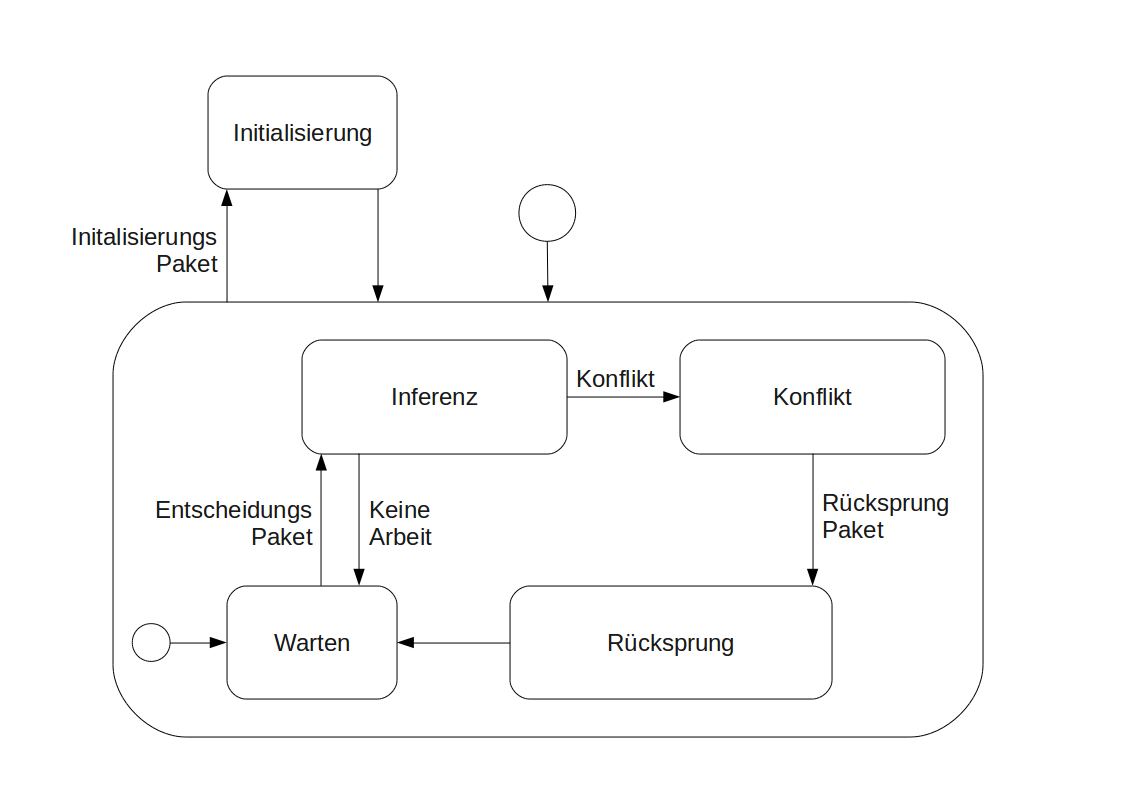
\includegraphics[width=\textwidth]{abb/state-chart.png}
  \caption{FPGA-Zustände}
  \label{modi}
\end{figure}

\subsection{Host-PC}
\label{host_pc}
Der Host-PC führt die softwareseitigen Komponenten (Gruppieren der Formel, Entscheidungsheuristik, 
Konfliktanalyse, Prüfen der Interpretation) des SAT-Solvers durch. 
Dabei kann man hierfür eigentlich jeden DPLL-Solver mit Rücksprung 
ohne Probleme anbinden. In Listing \ref{host_code} ist der benutzte Algorithmus des Host-PCs skizziert.
Es wird eine veränderte Form eines DPLL-Verfahrens genutzt.
Unterstrichen sind dabei die Funktionen, welche direkt mit dem FPGA interagieren.
\newpage
\lstset{
  language=C++, basicstyle=\small \ttfamily, showspaces=false, showtabs=false, tabsize=2 , keywordstyle=\bfseries, 
  showstringspaces=false, framexleftmargin=5mm, frame=single, numbers=left, numberstyle=\tiny, 
  stepnumber=1, numbersep=5pt, texcl=true, captionpos=b, commentstyle=\color{blue}, 
  classoffset=1,morekeywords={init,backtrack,propagate, wait}, keywordstyle=\color{red}\bfseries\underbar,
  classoffset=0}

\begin{lstlisting}[caption=Algorithmus Host-PC, label=host_code]
  
  // Der Algorithmus nimmt eine Formel
  // und gibt eine partielle Interpretation
  // zurück.
  vector<short int> dpll(Formula formula){

    int wait_result;             // Art des empfangenen Pakets
    vector<short int> decisions; // Entscheidungsliterale
    vector<short int> literals;  // Empfangene Literale 
                                 // vom FPGA
    vector<short int> trail;     // Partielle Interpretation
    short int lit = 0;           // Entscheidungsliteral
    short int backtrack_lit = 0; // Rücksprungliteral

    // Die Formel wird gruppiert und
    // an den FPGA geschickt.
    init(group(formula));

    while(1){
      // Warte auf eine Antwort des FPGAs.
      wait_result = wait(literals);

      // Aktualisiere die partielle Interpretation
      // mit den Daten des FPGAs.
      trail.push_back(literals);

      // Auswertung der FPGA-Antwort.
      // Das empfangene Paket ist unbekanntem Typs.
      if(wait_result == -1){
        return 0;
      }
      // Der FPGA hat einen Konflikt festgestellt
      // und muss zurückspringen.
      else if(wait_result == 2){
        backtrack_lit = backtrack(decisions, trail);
        propagate(backtrack_lit);
      }
      // Der FPGA braucht mehr Eingabedaten.
      // Das heißt die Entscheidung für eine
      // Variable muss getroffen werden.
      else if(wait_result == 3){
        lit = decide(interpretation, trail);
        if(lit != -1){
          propagate(lit);
        }
        else{
          // Keine weiteren Literale können entschieden werden.
          break;
        }
        decisions.push_back(lit);
      }
      // Der FPGA hat nur seine Daten geschickt,
      // da eine Sendefifo geleert werden musste.
      else if(wait_result == 4){
      }
    }

    return trail;
  }
\end{lstlisting}
Im Folgenden werden die unterstrichenen Funktionen im Quelltext von Listing \ref{host_code} erläutert:
\begin{itemize}
\item
  \textbf{Init(${\cal G}^{(1)}$)} initialisiert den FPGA, indem eine
  gruppierte Formel Literal für Literal über Ethernet an den FPGA gesendet
  wird. Das Ethernetpaket wird als Initialisierungspaket 
  markiert. Sollte eine neue Gruppe bzw. eine neue Klausel beginnen,
  werden diese Informationen durch bestimmte Steuerkodes im
  Ethernetpaket mitgesendet. Der Aufbau eines solchen
  Initialisierungspakets wird im Unterkapitel zur
  Ethernetschnittstelle beschrieben. Da der Entwurf für 9-SAT
  ausgelegt wurde, werden immer 9 Literale pro Klausel gesendet. 
  Sollte eine Klausel weniger als 9 Literale enthalten, wird 
  diese einfach mit Nullen aufgefüllt. Dies macht die Verarbeitung
  der Daten auf dem FPGA später einfacher, da man von einer 
  festen Klausellänge ausgehen kann.
\item
  \textbf{Propagate($l$)} sendet ein Literal $l$ über Ethernet an
 den FPGA. Das Paket wird als spezielles Entscheidungspaket
 markiert. Das Literal wurde normalerweise vorher durch
 eine Entscheidungsheuristik  bestimmt und war kein
 Element der partiellen Interpretation. Es wäre auch
 möglich, gleich mehrere Literale an den FPGA zu senden, 
 um weiteren Kommunikationsbedarf
 zu vermeiden. Das wäre der Fall,
  wenn nach vollständigem Propagieren weitere Literale angefordert
 werden. Jedoch würde dies
  eine kompliziertere Verwaltungslogik nach sich ziehen.
 So wurde sich bei diesem Entwurf dafür
  entschieden, nur ein Entscheidungsliteral senden und
 verarbeiten zu können.
\item
  \textbf{Backtrack(${l_1, …, l_n}$)} sendet eine Menge von Literalen über Ethernet an den FPGA
  und gibt das negierte letzte Entscheidungsliteral zurück. 
  Das Ethernetpaket wird als Rücksprungpaket markiert. Bei genutztem DPLL Algorithmus entsprechen
  die Literale der partiellen Interpretation bis zum letzten Entscheidungsliteral.\\
  Man könnte hier auch die Möglichkeit eines nonchronological Backtrackings (Backjumping) in 
  Betracht ziehen, wie es bei CDCL-Algorithmen angewandt wird. Dann müssten gelernte Klauseln
  in einer extra Datenstruktur auf dem Host-PC gehalten und separat propagiert werden.
  Außerdem müssten Unit-Literale der gelernten Klauseln dem FPGA mitgeteilt werden, was wieder mehr
  Kommunikationsbedarf bedeuten würde. 
  Die Rücksprungliterale werden auf dem FPGA ähnlich behandelt wie normale Literale, nur
  dass diese keinen Inferenzmechanismus auslösen und aus der partiellen Interpretation
  entfernt werden.

\item
  \textbf{Wait()} wartet auf eine Antwort des FPGAs. Ist das Antwortpaket mit dem 
  Steuerkode 0x02 markiert, dann handelt es sich um ein Konfliktpaket. 
  Alle Literal (jeweils 2\,Byte) die dem Steuerkode folgen sind Teile der partiellen 
  Interpretation und sollten zur partiellen Interpretation des Host-PCs 
  hinzugefügt werden, um diese zu aktualisieren. Das letzte Literal entspricht dabei dem Konflikt-Literal. 
  Ist das Antwortpaket mit 0x03 markiert, dann wartet der FPGA auf mehr Eingabedaten.
  Diese Eingabedaten sind Entscheidungsliterale und werden vom FPGA propagiert.
  Ist das Antwortpaket mit 0x04 markiert, dann wird eine Menge von Literalen gesendet, 
  welche der partiellen Interpretation hinzugefügt werden sollen. Dies geschieht 
  weil ein Sendefifo im FPGA geleert werden muss.
\end{itemize}
In Zeile 16 von Listing \ref{host_code} wird die Gruppierung der Formel F durchgeführt und
das Ergebnis an den FPGA gesendet. Je nach Größe des FPGAs und dem vorhandenen Block-RAM können verschieden viele Gruppen
erzeugt werden. Dabei gilt je mehr Gruppen verfügbar sind, desto größere Probleme kann man lösen.
Es gilt für $group: F \rightarrow {\cal G}^{(1)},\ |{\cal G}^{(1)}| = n$. Wobei die
Anzahl von möglichen Gruppen $n$ von FPGA-Parametern abhängt.\\

\subsection{Ethernet-Schnittstelle}
\label{ethernet}
Es gibt viele Möglichkeiten, um eine Kommunikation zwischen Host-PC
und FPGA zu realisieren. Dabei unterscheiden sie sich zum einen 
in ihrer Bandbreite und Latenz und zum anderen
im Aufwand ihrer Implementierung in Hardware. Sicher wäre eine
Verbindung über PCIe, HT etc. dem einer Ethernetschnittstelle vorzuziehen,
wenn es das Ziel ist, möglichst niedrige Kommunikationslatenzen zu erreichen.
Jedoch lassen sich diese Schnittstellen nur mit viel Aufwand implementieren,
so dass sich für den Prototyp für
Ethernet als Schnittstelle für den Entwurf entschieden wurde. 
Man kann das System auch sehr einfach durch weitere FPGA-Boards erweitern,
da diese nur an das Ethernetnetzwerk angeschlossen werden müssen.\\
Der Host-PC wird mithilfe einer Ethernet-Schnittstelle an den FPGA angebunden. 
Dabei wird ein bereits auf dem FPGA-Board vorhandener Ethernet-MAC-Schaltkreis genutzt. 
Die Kommunikation mit dem Ethernet-MAC erfolgt mittels Local-Link-Interface \cite{xilinxlocallink:2005}. 
Die übermittelten Pakete sind reine Ethernet-Pakete ohne weitere Schichten darüber 
wie Vermittlungs- bzw. Transportschicht. Ein Ethernet-Paket besteht aus einer Folge von 
minimal 64 bis maximal 1522\,Bytes. 
\begin{figure}[h]
  \centering
  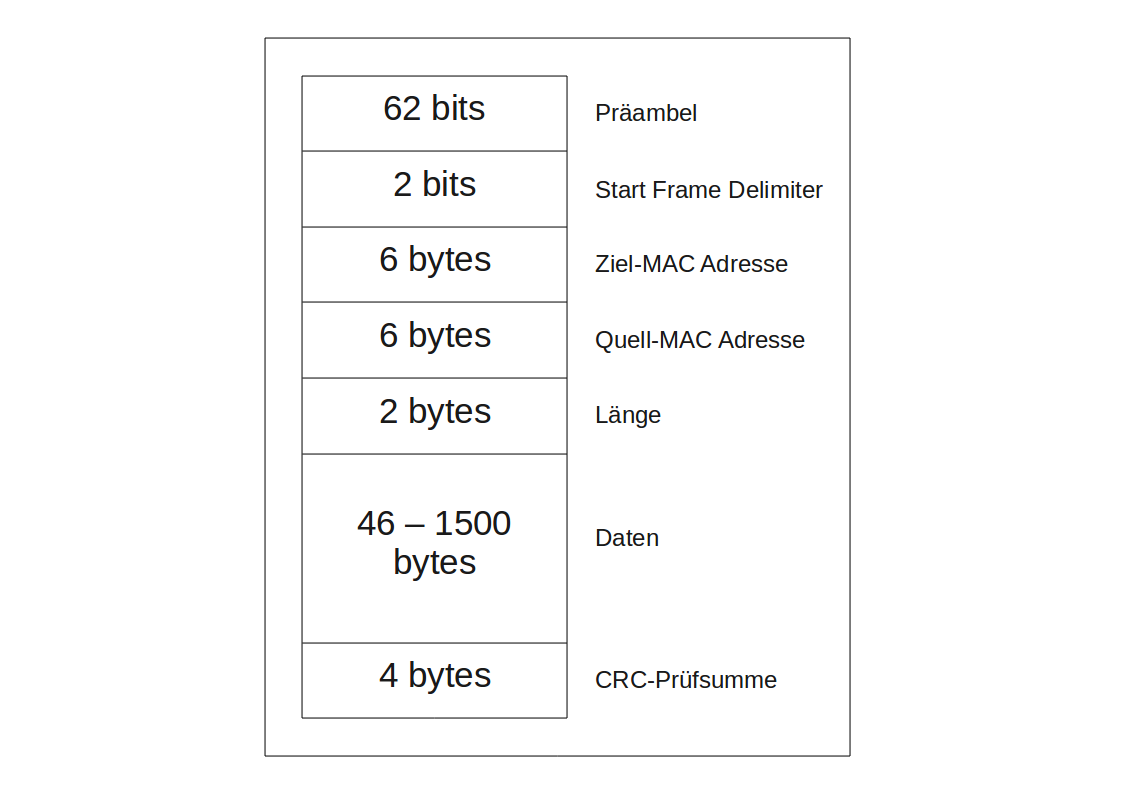
\includegraphics[width=0.75\textwidth]{abb/ethernet.png}
  \caption{Aufbau eines Ethernet-Pakets}
  \label{ether}
\end{figure}
Abbildung \ref{ether} zeigt den Aufbau eines Ethernet-Pakets,
wobei nur Ziel-MAC-Adresse, Quell-MAC-Adresse, Länge und die Daten vom Local-Link-Interface 
empfangen bzw. gesendet werden. Die restlichen Teile des Pakets werden vom 
Ethernet-MAC abgeschnitten bzw. hinzugefügt. Wie bereits im Host-PC-Kapitel erwähnt,  
werden Pakete mit speziellen Steuerkodes markiert um dem jeweiligen Empfänger 
(Host siehe Tabelle \ref{steuerkode2}, FPGA siehe Tabelle \ref{steuerkode1})
mitzuteilen, um welche Art von Paket es sich handelt. Der Steuerkode 
ist immer das erste Byte im Datenbereich des Pakets. Bytes werden in
der Byte-Reihenfolge Big Endian übertragen.
\begin{table}[h]
  \centering
  \begin{tabular}{|l|l|l|}
    \hline
    \textsc{Steuerkode} & \textsc{Bedeutung} & \textsc{Aufbau des Datenteils}\\
    \hline
    \hline
    $ 0x01 $ & Initialisierungspaket & 
    $\langle 0x01 \rangle,((\langle 0x0101 \rangle|\langle 0x0201 \rangle),l_1,l_2, ... , l_9)^+, $\\
    & & $\langle 0x0101 \rangle, (\langle 0x0000 \rangle)^9$\\
    $ 0x02 $ & Entscheidungspaket    & $\langle 0x02 \rangle,l$\\
    $ 0x03 $& Rücksprungpaket     & $\langle 0x03 \rangle ,l_1, ..., ln$\\
    \hline
  \end{tabular}
  \caption{Daten der Pakete vom Host-PC zum FPGA}
  \label{steuerkode1}
\end{table}
Der Aufbau des Initialisierungspakets ist etwas aufwändiger. Jede Klausel wird
Literal für Literal übertragen, jedoch wird vorher noch festgelegt, ob sich die nächste
Klausel in einer neuen Gruppe befindet (durch $0x0201$) oder ob die nächste Klausel in
der gleichen Gruppe ist wie die Klausel davor (durch $0x0101$). Deshalb
muss man darauf achten, die Gruppen in der richtigen Reihenfolge
zu übertragen. Ein Initialisierungspaket wird immer mit einer leeren Klausel
abgeschlossen.
\begin{table}[h]
  \begin{tabular}{|l|l|l|}
    \hline
    \textsc{Steuerkode} & \textsc{Bedeutung} & \textsc{Aufbau des Datenteils}\\
    \hline
    \hline
    $0x02$ & Konfliktpaket        & $\langle 0x02 \rangle (l)^*$\\
    $0x03$ & Eingabepaket         & $\langle 0x03 \rangle (l)^*$\\
    $0x04$ & Aktualisierungspaket & $\langle 0x04 \rangle (l)^*$\\
    \hline
  \end{tabular}
  \caption{Daten der Pakete vom FPGA zum Host-PC}
  \label{steuerkode2}
\end{table}
Die Pakete, welche der FPGA an den Host-PC sendet, ähneln sich im Aufbau sehr,
da mit jedem Paket auch Informationen über propagierte Literale an den 
Host-PC mitgesendet werden können. Die propagierten Literale sind Unit-Literale,
welche während des Inferenzprozessen auf dem FPGA entstanden sind. Die
Literale werden in einem Fifo zwischengespeichert und bei der nächsten 
Gelegenheit in einem Paket vom FPGA zum Host-PC mitgesendet.\\

\subsection{Literal-Arbiter}
\label{arbiter}
Arbiter kommt von \textit{to arbitrate} und heißt \textit{über etwas entscheiden}.
Das beschreibt die Funktion des Literal-Arbiters ganz gut, denn dieses
Modul entscheidet darüber, welches Literal als nächstes propagiert werden soll.
In Abbildung \ref{literal_arbiter} ist der Aufbau des Moduls grob skizziert. 
Signale von links entsprechen dabei Ausgangssignalen
des Ethernet-MAC-Moduls. Signale von rechts sind dementsprechend
Eingangs- bzw. Ausgangssignale der Propagation-Engines.\\
\begin{figure}[h]
  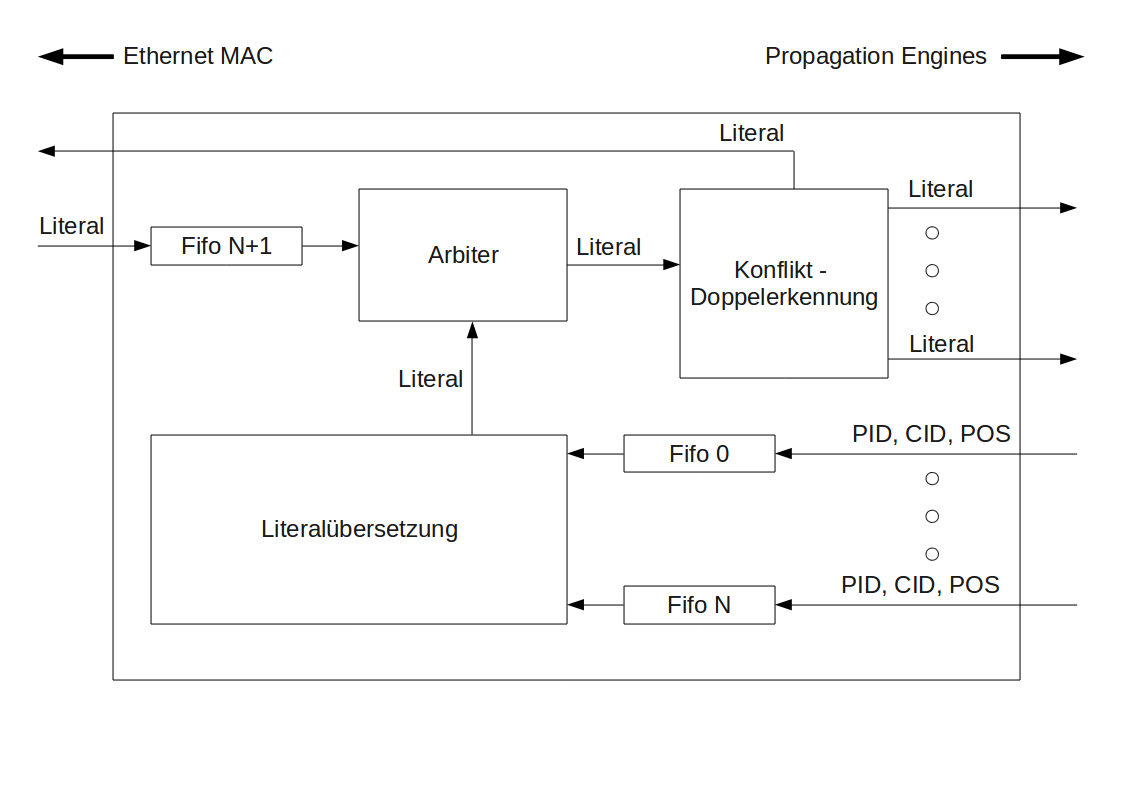
\includegraphics[width=\textwidth]{abb/literal_arbiter.png}
  \caption{Literal-Arbiter}
  \label{literal_arbiter}
\end{figure}Erläuterungen zu Abbildung \ref{literal_arbiter}:
\begin{itemize}
\item
  \textbf{FIFO N+1}\newline
  Dieser Fifo nimmt Entscheidungs- bzw. Rücksprungliterale vom Ethernet-MAC
  entgegen und speichert diese, bis sie weiter verarbeitet werden. Jedes
  Literal führt dabei die Information mit, ob es Entscheidungs- oder
  Rücksprungliteral ist.
\item
  \textbf{FIFO 0 bis N}\newline
  Diese Fifos speichern das Ausgangstupel(PID, CID, POS) von Signalen
  der jeweiligen Propagations- Engines 0 bis N. PID entspricht
  der Propagation-Engine-Identifikationsnummer und
  ist gleich dem Gruppenindex der zugehörigen Gruppe.\\
  CID entspricht der Klausel-Identifikationsnummer und ist innerhalb einer
  Propagation-Engine einmalig. POS entspricht der Position eines Literals innerhalb
  der Klausel, welche mit CID gekennzeichnet ist.
\item
  \textbf{Literal-Übersetzung}\newline
  Dem Tupel (PID, CID, POS) der Fifos 0 bis N werden 
  Literale zugeordnet, um mit diesen wieder Inferenz
  durchführen zu können. Welches Literal welchem Tupel
  zugeordnet wird entscheidet sich bei der Initialisierung
  des FPGAs. Sei die Formel
  $F_{group} = \langle[1,2],[2,3],[3,4],[4,5]\rangle$
  aus dem Gruppen-Einführungskapitel gegeben, dann wurde bereits festgestellt, dass man
  diese Formel in 2 Klauselmengen gruppieren kann. $G_1 = \{[1,2].[3,4]\}$, $G_2 = \{[2,3].[4,5]\}$.
  Zum Beispiel wird dem Literal $l = 2$ der ersten Klausel in $G_2$ das Tupel (2, 1, 1) zugeordnet.
  Die Zuordnungen werden im Block-RAM des FPGAs gespeichert. Bei
  32 Propagation Engines (5\,Bit), 128 Klauseln pro Propagation-Engine (7\,Bit) und
  9 Literalen pro Klausel (4\,Bit) ergibt sich eine 16\,Bit breite Adresse.
  Mit 9\,Bit pro Literal ergibt sich ein Gesamtspeicherbedarf von ca. 590\,kbit 
  ($2^{16}$ x $9$\,Bit) für die Literalübersetzungstabelle.

\item
  \textbf{Arbiter}\newline
  Der Arbiter entscheidet, welches Literal als nächstes propagiert werden soll
  und wählt dabei von den Fifos 0 bis N+1 aus. Es wird der Fifo ausgewählt, 
  welcher nicht leer ist und 
  den kleinsten Index hat. Somit werden Entscheidungsliterale immer
  zuletzt ausgewählt.

\item
  \textbf{Konflikt / Doppelerkennung}\newline
  Der Wahrheitswert jeder Variablen wird in einer partiellen Interpretation gespeichert. 
  Sollte ein Literal bereits interpretiert sein, dann gibt es zwei Möglichkeiten. Stimmt
  der Wahrheitswert des Literals mit dem der partiellen Interpretation überein, dann 
  muss das Literal nicht weiter bearbeitet werden, da es bereits propagiert wurde. 
  Sind die Wahrheitswerte gegensätzlich, dann wurde ein Konflikt gefunden, 
  welcher aufgelöst werden muss. Ein Konflikt wird dem Ethernet-MAC
  mitgeteilt, welcher wiederum den Host-PC informiert.
  Alle Literale, welche noch nicht in der partiellen Interpretation 
  des Host-PCs enthalten sind,
  werden an den Ethernet-MAC übermittelt. Dies ist notwendig, um den 
  Host-PC über den aktuellen Suchprozess zu informieren.
\end{itemize}

\subsubsection{Verhalten des Literal-Arbiters in \\ verschiedenen Zuständen}
Im Literal Arbiter wird prinzipiell zwischen fünf Zuständen unterschieden:
\begin{itemize}
\item
  \textbf{Initialisierungszustand}\\
  Im Initialisierungszustand wird keinerlei Inferenz durchgeführt, sondern nur Speicher initialisiert,
  welcher später von den Algorithmen gebraucht wird. Zum einen muss die Literal-Übersetzungstabelle 
  mit den entsprechenden (PID, CID, POS) zu Literalpaaren gefüllt werden, andererseits muss an die
  Propagation-Engine die Information übermittelt werden, welche Klauseln sie beinhalten. Die
  entsprechenden Signale werden über dedizierte Leitungen direkt in den Block-RAM
  der entsprechenden Module geschrieben.
\item
  \textbf{Inferenzzustand}\\
  Der Inferenzzustand ist der angenommene Normalfall, da es das Ziel
  des Systems ist, Inferenz durchzuführen. Literale werden vom Arbiter ausgewählt,
  von der Konflikt / Doppelerkennung getestet und dann an die Propagation-Engines übermittelt.
  In den Propagation-Engines werden dann die übermittelten Literale propagiert.
  Sollte ein Unit-Literal gefunden werden, dann wird dieses wieder inferiert.
\item
  \textbf{Rücksprungzustand}\\
  Der Rücksprungzustand verhält sich ähnlich zum Inferenzzustand nur das hier keine Konflikt und
  Doppelerkennung stattfindet, sondern die Wahrheitswerte der ausgewählten Literale werden in 
  der partiellen Interpretation auf undefiniert zurückgesetzt.
\item
  \textbf{Konfliktzustand}\\
  Sollte es innerhalb des Inferenzprozesses zu einem Konflikt kommen (erkannt durch
  die Konflikterkennung), dann wird die Bearbeitung weiterer Literale sofort eingestellt.
  Außerdem werden die Fifos 0 bis N+1 und die Fifos in den Propagation-Engines zurückgesetzt.
  Dieser ganze Prozess ähnelt einem Systemweiten Reset,  außer dass die Initialisierten
  Daten und die partielle Interpretation erhalten bleiben. Der Host-PC wird außerdem
  über die Konfliktsituation mit einem Konfliktpaket informiert und muss sich
  um die Konfliktbehandlung kümmern.
\item
  \textbf{Wartezustand}
  Wenn in keiner Propagation-Engine mehr ein Inferenzprozess stattfindet
  und der Literal-Arbiter keine Aufgabe hat, wechselt er in den Wartezustand.
  In diesem Zustand wartet er auf ein Entscheidungspaket vom Host-PC.
  Damit das der Host-PC weiß, wird er mit einem Eingabepaket informiert.
  
\end{itemize}

\subsection{Propagation-Engine}
\label{propagation_engine}
Das Propagation-Engine-Modul ist das eigentliche Herzstück des Entwurfs und führt 
die Inferenz von Literalen durch. Jeder Propagation Engine wird eine Gruppe zugewiesen.
Das heißt in einer Propagation Engine ist eine Variable maximal einmal
in einer Klausel vorhanden. In Abbildung \ref{pe} ist der Aufbau der Propagation Engine 
skizziert. Es werden zwei Hauptmodule unterschieden: das Literal-Lookup-Modul und das
Status-Tabellen-Modul.
\begin{figure}[h]
  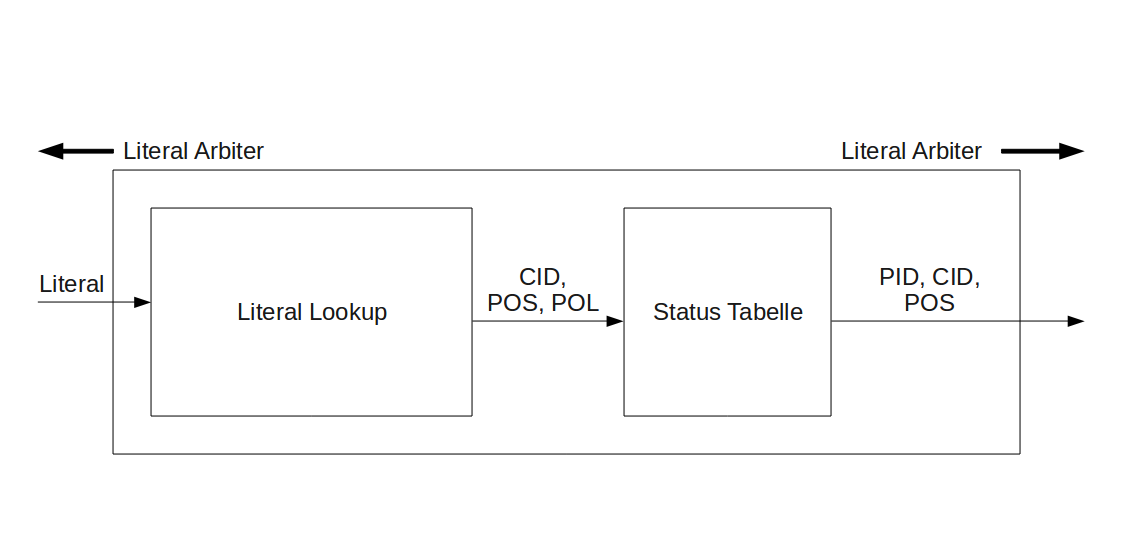
\includegraphics[width=\textwidth]{abb/propagation_engine.png}
  \caption{Propagation-Engine}
  \label{pe}
\end{figure}

\subsubsection{Literal-Lookup}
Das Literal-Lookup-Modul benutzt einen 18\,kbit Block-RAM. 
Damit ist es möglich, einen 10\,Bit Adressraum zu je 18\,Bit
Daten zu erzeugen. Eine Variable entspricht der Adresse des 
Block-RAMs und die Daten an dieser Adresse entsprechen der Klausel,
der Position und der Polarität des entsprechenden Literals (auch Wertetupel
der Variable genannt). Aufgabe des Literal-Lookup-Moduls
ist es, dieses Wertetupel an die Statustabelle weiterzugeben, 
falls es vorhanden sein sollte. Nicht vorhandene Wertetupel
sind im Speicher ausgenullt.
\begin{figure}[h]
  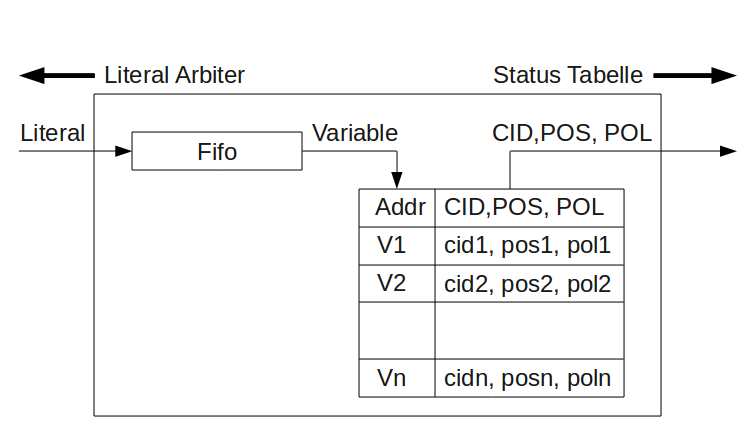
\includegraphics[width=0.75\textwidth]{abb/literal_lookup.png}
  \caption{Literal-Lookup}
  \label{literal_lookup}
\end{figure}
Somit ist die Anzahl der möglichen Variablen auf eine Obergrenze
von $2^{10}-1\ =\ 1023$ festgelegt (wobei die Literalübersetzung
die Variablenanzahl bereits auf 256 beschränkt). Literale werden in einem
Fifo gepuffert, so dass die Propagation-Engines unabhängig voneinander
arbeiten können. In Abbildung \ref{literal_lookup} ist das Literal-Lookup-Modul skizziert.


\subsubsection{Status-Tabelle}
Das Status-Tabellen-Modul benutzt ebenfalls einen 18\,kbit Block-RAM,
jedoch in einer Konfiguration mit einem 11\,Bit Adressraum zu je
9\,Bit Daten. Die Adresse des Block-RAMs entspricht der CID, welche
nur lokal für eine Propagation Engine gilt. Somit gibt es auch
eine Obergrenze von $2^{11} = 2048$ Klauseln pro Propagation Engine
(beschränkt auf 128 wegen Literalübersetzung).
Ein 9 Bit Datenwort entspricht der Interpretation
einer Klausel mit maximal 9 Literalen und wird hier Status genannt. Eine '0' an der Stelle m 
im Status bedeutet, dass das Literal an Position m unter der aktuellen
partiellen Interpretation den Wahrheitswert falsch zugewiesen bekommen hat.
Eine '1' an der Stelle m im Status bedeutet, das der Wahrheitswert des
Literals entweder wahr oder undefiniert ist. Dies wird nicht
unterschieden, da es keinerlei Information über mögliche Inferenz
liefert. Sollte eine Klausel weniger als 9 Literale enthalten, 
dann werden die restlichen Bits bereits beim initialisieren
vorgenullt. Wirklich existierende Literale werden im Status
Initial mit '1' belegt. In Abbildung \ref{status_tabelle}
ist das Status-Tabellen-Modul abgebildet.
\begin{figure}[h]
  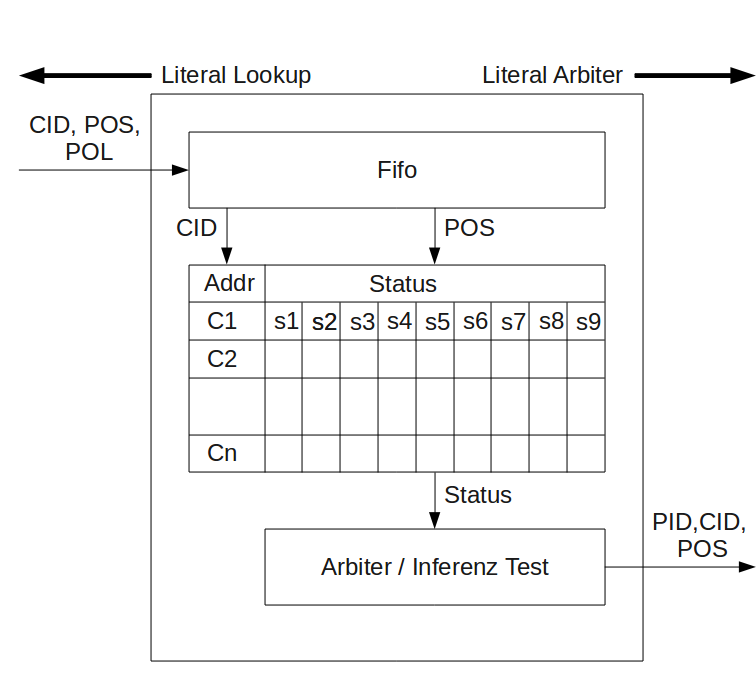
\includegraphics[width=0.75\textwidth]{abb/status_tabelle.png}
  \caption{Status-Tabelle}
  \label{status_tabelle}
\end{figure}

\subsubsection{Inferenz von Literalen}
Um nun herauszufinden, ob eine Klausel durch Propagieren 
eines Literals Unit wird, muss zuerst festgestellt werden, 
in welcher Klausel und an welcher Position sich das Literal
befindet (dies erledigt der Literal Lookup). 
Mit dieser Information kann der Status der Klausel aus dem 
Block-RAM geladen werden (da die Klausel-ID der Block-RAM Adresse
in der Status-Tabelle entspricht). An der Position des
Literals wird eine '0' im Status eingefügt, falls diese
noch nicht vorhanden ist, und es wird geprüft ob, der nun
entstandene Status nur noch eine '1' enthält. Diese Prüfung geschieht mittels
eines Arbiter-Moduls. Das Arbiter-Modul gibt die Position der ersten '1'
im Status als One-Hot-Code zurück. Wenn man nun den invertierten One-Hot-Code
mit dem Status verundet und eine Bitfolge von Nullen herauskommt,
dann wurde ein Unit Literal gefunden.\\
Sei nun wieder folgende Formel $F_{bsp}$ gegeben.
Dann kann diese Formel in 4 Klauselmengen gruppiert werden.
\begin{center}
$F_{bsp} = \langle [1,3],[-2, 5, -6], [-1,-4,6], [-1,-2,-4,5], [-1,2]\rangle$\\
$group(F_{bsp}) = \{\{[1,3],[-2,5,6]\},\{[-1,-4,6]\},\{[-1,-2,-4,5]\},\{[-1,2]\}\}$
\end{center}
Beispielhaft soll nun das Propagieren von zwei Literalen $l_1 = 2$, $l_2 = -5$ 
anhand der Propagation-Engine von Gruppe 1 
$(G_1 = \{[1,3],[-2,5,6]\})$ gezeigt werden. Es befinden sich $l_1$ und $l_2$ 
im Fifo des Literal-Lookup-Moduls und müssen propagiert werden.
Die Lookup-Tabelle von $G_1$ ist in Tabelle \ref{bsp_literal_lookup2} dargestellt.
%% \begin{table}[h]
%%   \centering
%%   \begin{tabular}{|c|c|c|c|}
%%     \hline
%%     \textsc{Variable} & \textsc{CID} & \textsc{POS} & \textsc{POL}\\
%%     \hline
%%     \hline
%%     1 & 1 & 1 & + \\
%%     \hline
%%     2 & 2 & 1 & - \\
%%     \hline
%%     3 & 1 & 2 & + \\
%%     \hline
%%     4 & - & - & - \\
%%     \hline
%%     5 & 2 & 2 & + \\
%%     \hline
%%     6 & 2 & 3 & + \\
%%     \hline
%%   \end{tabular}
%%   \caption{Literal-Lookup-Tabelle von Gruppe 1}
%%   \label{bsp_literal_lookup}
%% \end{table}
Die Wertetupel der Literale werden aus dem Speicher geladen
und an die Status Tabelle weiter geschickt. Die entsprechenden
Zeilen von $l_1$ und $l_2$ sind in Tabelle \ref{bsp_literal_lookup2}
durch Pfeile markiert.
\begin{table}[h]
  \centering
  \begin{tabular}{|c|l|l|l|}
    \hline
    \textsc{Variable} & \textsc{CID} & \textsc{POS} & \textsc{POL}\\
    \hline
    \hline
     1 & 1 & 1 & + \\
    \hline
    \textbf{$\rightarrow$ 2} & 2 & 1 & - \\
    \hline
    3 & 1 & 2 & + \\
    \hline
    4 & - & - & - \\
    \hline
    \textbf{$\rightarrow$ 5} & 2 & 2 & + \\
    \hline
    6 & 2 & 3 & + \\
    \hline
  \end{tabular}
  \caption{Ausgewählte Zeilen von $l_1$ und $l_2$}
  \label{bsp_literal_lookup2}
\end{table}
%\begin{center}
%  $l_1 \rightarrow (1, 1, +)$\\
%  $l_2 \rightarrow (2, 2, +)$
%\end{center}
Die initiale Status-Tabelle von Gruppe 1 ist in Tabelle \ref{bsp_literal_lookup3}
dargestellt. Der Status der ersten Klausel hat an Position eins und zwei eine '1'
- an den restlichen Position eine '0', da beide Literale der Klausel noch
undefiniert sind. Analog dazu hat auch die zweite Klausel an erster bis dritter
Position eine '1' im Status.
\begin{table}[h]
  \centering
  \begin{tabular}{|c|l|l|l|l|l|l|l|l|l|}
    \hline
    \textsc{CID} & \textsc{1} & \textsc{2} & \textsc{3}& \textsc{4}& \textsc{5}& \textsc{6}& \textsc{7}& \textsc{8}& \textsc{9}\\
    \hline
    \hline
    1 & 1& 1& 0& 0& 0& 0& 0& 0& 0 \\
    \hline
    2 & 1& 1& 1& 0& 0& 0& 0& 0& 0 \\
    \hline
  \end{tabular}
  \caption{Status-Tabelle von Gruppe 1}
  \label{bsp_literal_lookup3}
\end{table}
Die Wertetupel von $l_1$ und $l_2$ werden nun auf die Statustabelle
angewandt (siehe Tabelle \ref{bsp_literal_lookup4}).
Das heißt in Zeile 2 der Statustabelle werden Positionen eins und zwei genullt.
Das Ergebnis ist der Status (001000000). Der Arbiter gibt nun die Position
der ersten '1' als One-Hot-Code zurück (001000000). Verundet man den negierten 
One-Hot-Code mit dem Status erhält man (000000000), was bedeutet, dass
an Position 3 dieser Klausel ein Unit-Literal gefunden wurde.
\begin{table}[h]
  \centering
  \begin{tabular}{|c|l|l|l|l|l|l|l|l|l|}
    \hline
    \textsc{CID} & \textsc{1} & \textsc{2} & \textsc{3}& \textsc{4}& \textsc{5}& \textsc{6}& \textsc{7}& \textsc{8}& \textsc{9}\\
    \hline
    \hline
    1 & 1& 1& 0& 0& 0& 0& 0& 0& 0 \\
    \hline
    2 & \textbf{0}& \textbf{0}& 1& 0& 0& 0& 0& 0& 0 \\
    \hline
  \end{tabular}
  \caption{Status-Tabelle von Gruppe 1 nach propagieren von $l_1$ und $l_2$}
  \label{bsp_literal_lookup4}
\end{table}
Es ist noch nicht bekannt, um welches Literal es sich genau
handelt, man weiß nur sein Identifikationstupel (PID,CID,POS).
Für eine weitere Inferenz des gefundenen Unit-Literals
wird das Tupel (1,2,3) an den Literal-Arbiter weitergeleitet
und dort zurückübersetzt. Man weiß das sich in
der ersten Gruppe in der zweiten Klausel an dritter Position
ein Unit Literal befindet.


%%% RESULTATE %%%%%%%%%%%%%%%%%%%%%%%%%%%%%%%%%%%%%%%%%
\section{Resultate}
Sowohl in \cite{davis:2008} als auch in \cite{haller:2010} wurden zwar
vielversprechende Ansätze für Hardware-SAT-Solver vorgestellt, 
jedoch fehlen beiden Arbeiten ernstzunehmende Resultate,
da sie entweder  nur den Entwurf simulieren 
und nicht das Gesamtsystem betrachten oder ganz fehlen.
In den folgenden Abschnitten werden Resultate des
vorgestellen Enwurfs diskutiert.

\subsection{Synthese des Entwurfs}
Zur Umsetzung des Entwurfes stand ein Xilinx ML505
Entwicklerboard \cite{xilinxml505:2011} mit einem Virtex-5
XC5VLX50T FPGA \cite{xilinxvirtex5:2009} zur Verfügung .
Für den Entwurf wurde die Ethernet PHY Schnittstelle und
der FPGA auf dem Entwicklerboard benutzt.
Auf dem FPGA-Chip sind 7200 Logikzellen mit je 4 LUTs und FlipFlops, 
60 x 36\,kbit Block-RAM (oder 120 x 18\,kbit),
480 kbit Distributed-RAM und 4 Ethernet-MACs vorhanden.\\
Für diesen FPGA kann ein Entwurf mit 32 Propagation-Engines, 128 Klauseln in 9 SAT pro
Propagation Engine und 256 Variablen synthetisiert werden. Der Schaltkreis wird mit
125\,MHz getaktet. Man könnte ihn sogar noch höher takten (ca. 250\,MHz), jedoch wurde zwecks einfacher
Kommunikation mit dem Ethernetmodul darauf verzichtet.
Die Synthese wurde mithilfe von ISE in Version 10.1.02 (lin64) durchgeführt.
Eine Zusammenfassung über die benötigten Ressourcen des synthetisierten Schaltkreises findet man in 
Tabelle \ref{ressources}.
\begin{table}[h]
  \begin{tabular}{|l|l|l|l|}
    \hline
    \textsc{Logikelement} & \textsc{Benutzt} & \textsc{Verfügbar} &\textsc{Ausnutzung}\\
    \hline
    \hline
    LUTs & 10053 & 28800 & 34\%\\
    \hline
    davon LUTs als Logik & 8348 & - & -\\
    \hline
    davon LUTs als Speicher & 1698 & - & -\\
    \hline
    FlipFlops & 5701 & 28800 & 19\%\\
    \hline
    Block-RAM & 53 & 60 & 88\%\\
    \hline
    davon 18\,Kbit Block-RAM & 70 & - & -\\
    \hline
    davon 36\,Kbit Block-RAM & 18 & - & -\\
    \hline
  \end{tabular}
  \caption{Ressourcenverbrauch des Entwurfs auf Virtex 5 X50T}
  \label{ressources}
\end{table}
Der Flaschenhals des Entwurfs liegt eindeutig im Verbrauch von Block-RAM.
Die 32 Propagation-Engines brauchen 64 x 18\,kbit Block-RAM und die
restlichen 18 x 36\,kbit und 6 x 18\,kbit Block-RAMs werden vom 
Literal-Übersetzungs-Modul benutzt. Die Lookup-Tabellen des FPGAs sind
nur zu 34\% ausgelastet, so dass noch viel Platz für Logik vorhanden ist
und auch die FlipFlops der LUTs sind nur mäßig belegt.


\subsection{Experimente}
In diesem Unterkapitel soll der in dieser Arbeit entstandene 
FPGA-SAT-Solver mit einem Software-Solver verglichen werden.
Der Software-Solver ist ein reiner DPLL-Solver und 
verhält sich exakt so wie der FPGA-Solver. 
Das heißt, es werden die gleichen Entscheidungen getroffen
und bei Konflikten wird der gleiche Rücksprungpunkt bestimmt,
so dass die Solver den gleichen Suchbaum erzeugen.
Nur die benutzten Algorithmen zur 
Umsetzung des Inferenzprozesses sind unterschiedlich.
Der Software-Solver sucht im Inferenzprozess jede Klausel
nach möglichen Unit-Literalen ab.\\
Um die Unterschiede zwischen Software- und 
Hardware-SAT-Solver zu verdeutlichen wurden
drei Testfälle ausgewählt:
\begin{itemize}
  \item 
    \textbf{Testfall 1} besteht aus einer Menge von Formeln mit maximal 32 Klauseln,  
    welche durch das Propagieren von Literal $l = -1$ gleichzeitig Unit werden und somit 
    den Inferenzprozess anstoßen. Mehr als 32 Klauseln können nicht
    gleichzeitig getestet werden, da der FPGA nur bis zu 32
    Gruppen unterstützt. Dieser Test wurde ausgewählt um die parallele Leistungsfähigkeit
    der Solver zu testen.
  \item
    \textbf{Testfall 2} besteht aus einer Menge von Formeln mit maximal
    100 Klauseln, wobei durch Propagieren von Literal $l = -1$ eine
    Inferenzkette von Unit-Literalen entsteht.
    Mit diesem Test wird geprüft wie die Leistungsfähigkeit die Solver bei
    der seriellen Abarbeitung von Literalen sind.
  \item
    \textbf{Testfall 3} besteht aus ausgewählten Instanzen
    der SATLIB \cite{satlib:2003} und einer kleinen Instanz der SAT-Competition \cite{satcomp:2011}. 
    Diese Probleme wurden ausgewählt, um die Leistung der Solver
    bei bereits vorhandenen Problemen zu vergleichen.
\end{itemize}
Im getesteten System sollen alle Faktoren mit
eingerechnet werden. So werden auch die 
Ethernetübertragungszeiten nicht vernachlässigt, da
sie einen Großteil der benötigten Zeit stellen.
Die Zeit die der FPGA benötigt, um ein Literal
zu propagieren ist fast vernachlässigbar. Er braucht
genau 76 Takte, dass entspricht 608\,ns bei
einer Taktfrequenz von 125\,MHz. In den 76 Takten 
sind bereits die Ethernetverabeitungszeiten
enthalten. Für das Senden eines Pakets muss
man dann nocheinmmal ca. 300\,$\mu$s veranschlagen.
In den Experimenten 1 bis 3 werden jeweils
die Anzahl der gesendeten Pakete angegeben.
Außerdem muss bedacht werden, dass
die Software des Host-PCs auch noch 
Zeit braucht. Diese Zeit ist jedoch schwer
zu bestimmen, da sie von der momentanen Auslastung
des Hostsystems abhängt. Der bei den Experimenten
genutzte Host-PC ist ein Intel Core 2 Quad 2.6\,GHz 
64\,Bit mit 8\,Gbyte Hauptspeicher.



\subsubsection{Parallele Inferenz von Literalen}
In diesem Testfall soll die parallele Leistung
von Software- und Hardware-SAT-Solver gemessen
werden, um zu zeigen, welche Auswirkungen die
verschiedenen Inferenzalgorithmen auf
das Zeitverhalten haben. Es wurden 9 Formeln 
mit jeweils 1, 4, 8, 12, 16, 20 , 24, 28 und 32
Klauseln ausgewählt. Diese Klauseln werden Unit wenn das Literal
$l = -1$ propagiert wird, wobei alle Unit-Literale unterschiedlich sind.
\begin{center}
      $F_{Test1\ [32]} = \langle [1,2],[1,3],...,[1,32],[1,33]\rangle$
\end{center}
In der Laufzeit des FPGA Solvers werden 
3 Ethernetpakete verschickt (Initialisierungs-, Entscheidungs-,
Eingabepaket).
Das Zeitverhalten in Abhängigkeit von
der Anzahl der Klauseln wird in Abbildung \ref{parallelinferenz}
grafisch dargestellt.
\begin{figure}[h]
  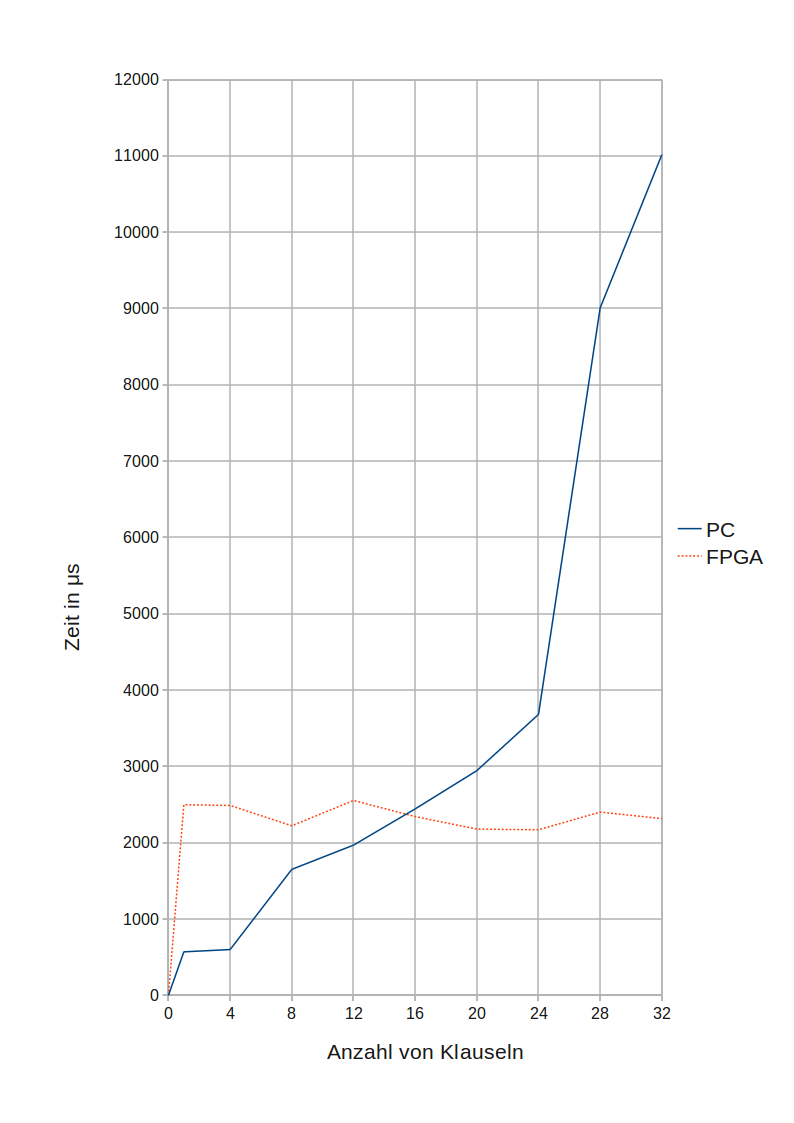
\includegraphics[width=0.65\textwidth]{abb/testfall1.png}
  \caption{Parallele Inferenz von Literalen}
  \label{parallelinferenz}
\end{figure}
Man erkennt in Abbildung \ref{parallelinferenz} gut, dass obwohl sich
die Anzahl der Klauseln erhöht, die Zeit welche der FPGA-SAT-Solver benötigt, 
um die Formel zu lösen, stets konstant bleibt. Diese Eigenschaft lässt sich
leicht erklären. Da alle 32 Propagation-Engines parallel arbeiten und sich
alle Klauseln in verschiedenen Gruppen befinden, können auch alle
Klauseln gleichzeitig propagiert werden.
Im Schnitt benötigt der FPGA Solver also 2,5\,ms, wovon 0,9\,ms auf das
Versenden von Paketen zurückzuführen sind. Die restliche Zeit
benötigt der Host-PC für seine Berechnungen.\\
Im Gegensatz dazu steigt die benötigte Zeit des Software Solvers
mit zunehmender Klauselanzahl stark an. Dies 
ist darauf zurückzuführen, dass der Software-Solver
Literale nicht parallel verarbeiten kann.

\subsubsection{Serielle Inferenz von Literalen}
Auch die serielle Leistung der Solver muss verglichen werden.
Hierfür eignet sich eine Formel mit Inferenzkette. Das heißt, jedes
Unit-Literal erzeugt in einer anderen Klausel wiederum ein Unit-Literal und so weiter.
Es wurden 8 Formeln mit jeweils 1, 4, 8, 16, 32, 64, 80 und
100 Klauseln getestet. 
    \begin{center}
      $F_{Test2} = \langle [1,2],[-2,3],[-3,4],[-4,5][-5,6],...,[-100,101]\rangle$\\
      $Inferenzkette:\ \ \ \ \ \ \ -1 \rightarrow 2 \rightarrow 3 \rightarrow 4 \rightarrow ... \rightarrow 100 \rightarrow 101$
    \end{center}
Für die Formeln mit 1 bis 64 Klauseln
werden 3 Pakete für den FPGA Solver benötigt (Initialisierungs-, Entscheidungs-, Eingabepaket).
Die Formeln mit 80 bzw. 100 Klauseln benötigen 1 Paket
mehr, da die Formel nicht mehr allein in ein Initialisierungspaket passt.
\begin{figure}[h]
  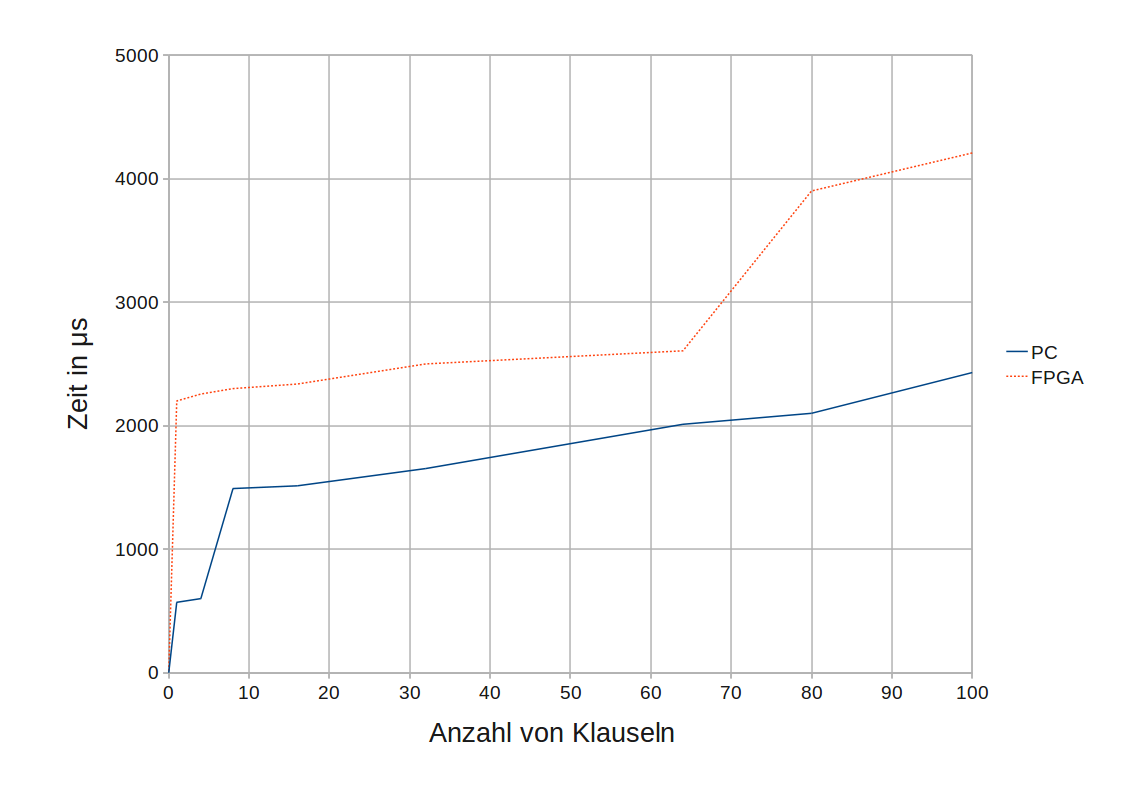
\includegraphics[width=\textwidth]{abb/testfall2.png}
  \caption{Serielle Inferenz von Literalen}
  \label{seriellinferenz}
\end{figure}
In Abbildung \ref{seriellinferenz} ist zu erkennen, dass der FPGA-Solver stets mehr
Zeit benötigt als die Software-Lösung. Der Zeitanstieg in
Abhängigkeit zur Anzahl von Klauseln ist jedoch gleich. Der PC ist zwar
mehr als 10 mal so hoch getaktet wie der FPGA, jedoch braucht der
FPGA weniger als ein Zehntel der Zeit, um ein Literal zu propagieren.
Somit gleichen sich Hardware- und Softwarelösung im seriellen Vergleich
aus. Für die größeren Lösungszeiten sorgt letztendlich nur
die Ethernetkommunikation. Ab 80 Klauseln benötigt der FPGA-Solver
plötzlich mehr Zeit. Diese Zeit ist auf das zusätzliche
Ethernetpaket zurückzuführen, welches gesendet werden muss.


\subsubsection{Lösen von ausgewählten Problemen}
Natürlich bestehen SAT-Probleme nicht nur aus paralleler
bzw. serieller Inferenz sondern aus einer Mischung von
beidem. Dazu kommt noch, dass die Entscheidungsheuristik
eines SAT-Solvers nicht immer richtig liegt und der
Suchprozess früher oder später in einem Konflikt endet.
Um Konflikte zu lösen, muss der FPGA-SAT-Solver wieder
Pakete verschicken, wobei sich gezeigt hat, dass sich dies
negativ auf die Laufzeiten auswirkt.
\begin{table}[h]
  \centering
  \begin{tabular}{|l|l|l|l|}
    \hline
    \textsc{Instanz} & \textsc{Variablen} & \textsc{Klauseln} &\textsc{Gruppen}\\
    \hline
    \hline
    anomaly.cnf & 48 & 261 & 22\\
    \hline
    flat-easy-1.cnf & 90 & 300 & 8\\
    \hline
    289-sat-4x8.cnf & 128 & 896 & 25\\
    \hline
  \end{tabular}
  \caption{Daten ausgewählter Probleme}
  \label{problems_data}
\end{table}
Anhand von SAT-Instanzen aus der SATLIB \cite{satlib:2003} und
SAT-Competition \cite{satcomp:2011}
sollen Hardware- und Software-Solver unter realen 
Bedingungen verglichen werden. Bei den Instanzen handelt es
sich um ein Planungsproblem (Blocks World:anomaly.cnf), 
ein Graphfärbeproblem (Graph Coloring:Flat Easy:flat-easy-1.cnf) 
und ein Problem unbekanntem Typs (289-sat-4x8.cnf).
In Tabelle \ref{problems_data} werden Eigenschaften der Problemdateien
aufgelistet. Ergebnisse findet man in Tabelle \ref{problems}. Wobei die Laufzeiten
Durschnittswerte aus mehreren Durchläufen sind.
\begin{table}[h]
  \centering
  \begin{tabular}{|l|l|l|l|l|}
    \hline
    \textsc{Instanz} & \textsc{Laufzeit PC} & \textsc{Laufzeit FPGA} &\textsc{ges. Pakete}&\textsc{Sendezeit}\\
    \hline
    \hline
    anomaly.cnf & 6,1\,ms & 10,2\,ms & 17 & 5,1\,ms\\
    \hline
    flat-easy-1.cnf & 8,2\,ms & 22,0\,ms & 53 & 15,9\,ms\\
    \hline
    289-sat-4x8.cnf & 22,6\,ms & 60,7\,ms & 129 & 38,7\,ms\\
    \hline
  \end{tabular}
  \caption{Ergebnisse ausgewählter Probleme}
  \label{problems}
\end{table}
\newpage
Dabei werden folgende Instanzen unterschieden:
\begin{itemize}
  \item
    \textbf{anomaly.cnf}\\
    Das Problem lässt sich in 22 Gruppen gruppieren und kann somit vom FPGA-Solver
    gelöst werden. Er braucht 10,237\,ms und somit ca. 4\,ms mehr als der Software
    Solver. Die Ethernetsendezeit beträgt 5,1\,ms und somit die Hälfte der gesamten
    Laufzeit.

  \item
    \textbf{flat-easy.cnf}\\
    Für dieses Problem werden nur 8 Gruppen benötigt und es kann somit auch ohne weiteres
    vom FPGA-Solver gelöst werden. Es müssen 53 Ethernetpakete zur Kommunikation
    zwischen Host und FPGA verschickt werden. Das sind wesentlich mehr als bei
    anomaly.cnf, was sich auf die Laufzeit des FPGA-Solvers auswirkt. Die Softwarelösung
    benötigt 14\,ms weniger Zeit als der FPGA, wobei 15,9\,ms der FPGA-Lösungszeit
    von der Paketsendung verbraucht wird.
\item
    \textbf{289-sat-4x8.cnf}\\
    Bei dieser Problemdatei handelt es sich um die größte Formel der
    ausgewählten Instanzen. Zieht
    man von der Lösungszeit des FPGA-Solvers die Zeit, welche
    für das versenden der Pakete gebraucht wird ab, dann lösen
    beide Solver die Problemdatei in der gleichen Zeit.

\end{itemize}
\subsection{Fazit}
In diesem Abschnitt sollen nochmal alle Testfälle zusammengefasst
werden, um daraus ein Fazit ziehen zu können. So hat sich durch
Testfall 1 gezeigt, dass der FPGA-SAT-Solver Literal besser
parallel verarbeiten kann, denn Literale werden in den einzelnen
Gruppen alle gleichzeitig propagiert. Bei der seriellen Inferenz, 
in Testfall 2, schneiden FPGA- und Software-SAT-Solver etwa gleich ab, wobei
der FPGA-Solver mit einem Ethernet-Overhead zu kämpfen hat.
Parallele und serielle Inferenz wurden in Testfall 3 bei
realen Problemen sozusagen gemischt. Bei allen Problemen
ist der Software-Solver klar schneller, da der Solver nicht 
mit einem FPGA kommunizieren muss. Der FPGA-SAT-Solver konnte
jedoch nicht sein volles Potential ausschöpfen, weil
es schwierig ist große Formel zu finden,
welche, trotz der vielen Beschränkungen, lösbar sind. Denn selbst
wenn Variablen und Klauselanzahl unter den Möglichkeiten bleiben, 
muss es nicht gezwungenermaßen möglich sein, 
eine Gruppierung für 32 Gruppen durchzuführen.
Bei allen Problemdateien könnte der FPGA-Solver,
durch eine schnellere Kommunikation zum Host-PC, an die Lösungszeiten
des Software-Solvers herankommen.
Denn bei geringerer Kommunikationlatenz oder
besserer Verschränkung der Kommunikation zwischen FPGA und Host-PC, ist eine
Verbesserung der Lösungszeit
durchaus denkbar. 
Einen klaren Vorteil hat die Software-Lösung
in Hinsicht auf die Problemgröße der SAT-Instanzen. Dem 
Software-Solver steht ein großer DRAM-Speicher zur Verfügung, welcher
wesentlich mehr als 256 Variablen und 4096 Klauseln zulässt.\\
Schlussendlich kann man sagen, das der Software-Solver
bei den getesteten Problemen stets die bessere Wahl ist. Jedoch
gibt es Möglichkeiten Performance und Ressourcenausnutzung
des FPGA-SAT-Solvers zu verbessern. Einige dieser Möglichkeiten werden im
folgenden Abschnitt näher betrachet.








%%% Zukünftige Arbeit %%%%%%%%%%%%%%%%%%%%%%%%%%%%%%%%%
\section{Zukünftige Arbeit}
Es gibt einige Möglichkeiten den vorgestellten Entwurf
zu verbessern und zu erweitern. Denn um mit modernen SAT-Solvern
mithalten zu können, muss die Anzahl möglicher Variablen
weiter erhöht werden. Auch über eine bessere Kommunikation zwischen
FPGA und Host-PC muss man nachdenken (Abschnitt \ref{kommu}).\\
Ein klarer Schwachpunkt im Entwurf ist der Speicherverbrauch.
So beschränken die Literal-Lookup-Tabellen, durch ihren 
einfachen Aufbau, die Variablenanzahl auf 1024 mögliche Variablen.
Noch viel stärker wird die Variablenanzahl durch die 
Übersetzungstabelle im Literal-Arbiter eingeschränkt (256 Variablen).
Obwohl 2048 Klauseln pro Propagation-Engine
möglich wären, wird auch deren Zahl durch die Übersetzungstabelle
auf 128 Klauseln pro Propagation-Engine begrenzt. Aus der Tatsache,
das der Block-RAM-Speicher knapp ist, folgt außerdem, das maximal 32 Propagation-Engines
erzeugt werden können, was die lösbaren Problemdateien weiter
einschränkt.\\
In der Arbeit von Davis \cite{davis:2008} ist es dem FPGA-SAT-Solver
möglich bis zu $2^{16}$ Variablen und Klauseln bei maximal 64
Gruppen zu verarbeiten. Sie verwenden einen Xilinx Virtex-5 
XC5VLX110T FPGA mit mehr als doppelt soviel Block-RAM (296 x 18Kbit).
Die Literal-Übersetzungstabelle wird komplett in einem
DRAM gespeichert, so dass alle Block-RAMs für die Propagation-Engines
zur Verfügung stehen. Statt einer einfachen Literal-Lookup-Tabelle
benutzt Davis einen Baum im Block-RAM-Speicher, 
um Variablentupel wiederzufinden. Dieser Baum macht es möglich
wesentlich mehr Variablen zu referenzieren. 
Eine weitere Möglichkeit, die Lösungszeit des FPGA-Solvers
zu optimieren, ist es statt des DPLL-Algorithmus den CDCL-Algorithmus zu
nutzen. Welche Möglichkeiten der CDCL-Algorithmus bietet,  
wird in Abschnitt \ref{cdcl} diskutiert.
Wie der Entwurf erweitert werden kann, 
um größere Formeln zu lösen, wird in Abschnitt \ref{bigformula} 
vorgestellt. In Abschnitt \ref{treelookup} wird der bereits
angesprochene baumstruckturierte Literal-Lookup erläutert.

\subsection{Lösen größerer Formeln}
\label{bigformula}
Die lösbare Formelgröße wird primär durch den verfügbaren
Speicher in der Literal-Übersetzungstabelle bestimmt.
Denn eigentlich entspricht der Inhalt der Tabelle der
vollständigen Formel. Jedem Literal wird darin seine
Gruppe, Klausel und Position zugewiesen, was einer
eindeutigen Positionsbestimmung innerhalb der Formel
gleichkommt. Je mehr Speicher in der 
Literal-Übersetzungstabelle zur Verfügung steht, um so
größere Formeln können gelöst werden. Im 
vorgestellten Entwurf steht dieser Tabelle
nur ein Teil des Block-RAMs des FPGAs zur Verfügung, so
dass nur kleine Formeln lösbar sind. Auf dem
genutzten ML505-Board exisitiert jedoch ein 9 Mbit
großer SRAM-Speicher (256k x 36 Bit). Es besteht
die Möglichkeit die Übersetzungstabelle in den 
vorhandenen SRAM-Speicher auszulagern.
So könnte man 64 Gruppen (6 Bit), 1024 Klauseln
(10 Bit) pro Gruppe und 8 Literale (3 Bit) pro 
Klausel realisieren. Mit 17 Bit pro Literal
ergibt sich ein ein Gesamtspeicherbedarf
von ca. 8,9 Mbit ($2^{19}$ x 17 Bit). Die 8,9 Mbit große 
Übersetzungstabelle passt vollständig in den 
SRAM-Speicher des Entwicklerboards.\\
Desweiteren wird die Problemgröße durch
die Literal-Lookup-Tabellen in den
Propagation-Engines bestimmt. Eine
Literal-Lookup-Tabelle kann maximal
auf 1024 Variablentupel zeigen, was
bedeutet, dass die Variablenanzahl 
auf maximal 1024 Variablen pro
Formel begrenzt wird. Im folgenden
Abschnitt wird ein baumstruckturierter
Literal-Lookup diskutiert, um dieses
Problem zu lösen.





%Da es sich bei der Literal Übersetzungstabelle um eine große Matrix handelt,
%könnte man diese in dem auf ML505 Board vorhandenen SRAM auslagern um mehr Block Ram 
%für die Propagation Engines zur Verfügung zu haben




\subsection{Ein baumstruckturierter Literal-Lookup}
\label{treelookup}
In diesem Unterkapitel wird eine Technik diskutiert,
mit der man die Anzahl möglicher Variablen im 
Entwurf erhöhen kann. Denn Probleme, welche moderne
SAT-Solver lösen können, haben bis zu mehreren 
Millionen Variablen und Klauseln\\
Das bisherige Literal-Lookup-Tabellen-Modul einer Propagation-Engine
entspricht einer einfachen Lookup-Tabelle. Das heißt,
wenn $M$ Speicherplätze (Adressen) in einem Block-RAM zur
Verfügung stehen, dann können auch nur $2^k-1 = M$ Variablen unterstützt werden,
da eine Adresse des Speichers dem Wert einer Variablen entspricht. 
Davon ausgehend, dass nicht jede unterstützte Variable in einer Gruppe vorhanden
ist, könnte die Anzahl der unterstützten Variablen $2^k$ wesentlich 
größer sein als die Anzahl der Speicherplätze $M$ in einem
Block-RAM, so dass gilt $M < 2^k$. Die einfachste Art, so etwas zu realisieren, wäre
eine Hashtabelle wobei die Variable der Schlüssel sowie Klausel, Position und
Polarität die zugehörigen Werte wären. Das Hardwareäquivalent einer Hashtabelle
wird Assoziativspeicher oder auch inhaltsadressierbarer Speicher 
(engl. Content Adressable Memory CAM) genannt.\\
Davis \cite{davis:2008} verzichtet auf Assoziativspeicher, da
diese auf den meisten FPGAs nicht vorhanden sind. Deshalb 
wird im Block-RAM ein Baum aufgebaut, welcher dafür sorgt, dass
für eine Variable die entsprechenden Wertetupel gefunden werden.\\
Die Frage ist, wie ein solcher Baum aufgebaut ist, wie
man ihn herstellen und wie darin das gesuchte Tupel
einer Variable gefunden werden kann. Es folgt eine Beschreibung
von Eigenschaften des Baumes.
Jeder Knoten des Baumes verbraucht einen Speicherplatz im Block-RAM.
Also kann man den verbrauchten Speicherplatz des Baumes anhand der
benutzten Knoten ermitteln.
Die Blätter des Baumes sind entweder Tupel von der Form (CID, POS, POL)
oder werden als leer markiert. 
Jeder Knoten, welcher kein Blattknoten ist hat $2^m$ Kindsknoten und beinhaltet eine Basisadresse. 
Eine Variable kann mit k Bitstellen binär dargestellt werden (somit ergibt sich eine Gesamtzahl
von $2^k-1$ Variablen). Der Baum hat eine maximale Tiefe von $k/m$.\\
Um nun das gesuchte Tupel einer Variable im Baum zu finden 
beginnt man bei Basisadresse 0x0 und teilt die binär dargestellte Variable in $k/m$ teile.
Dann addiert man binär den ersten Teil der geteilten Variable zur Basisadresse hinzu und erhält
die Adresse an welcher sich die neue Basisadresse befindet. Dieser Vorgang wird solange wiederholt
bis man zum letzten Teil der geteilten Variable gelangt. Addiert man jetzt noch einmal den
letzten Teil der Varibale ist
der Inhalt im Speicher an der neuen Basisadresse unser gesuchtes Tupel. Sollte man zwischendurch auf einen 
leeren Knoten stoßen, dann gibt es für diese Variable keine zugehörige Klausel in diesem Baum
und der Prozess kann abgebrochen werden. Ein Spezialfall wäre $k = m$, dann
würde der Baum der Lookup-Tabelle im vorgestellten Entwurf entsprechen.\\
In Abbildung \ref{tree} wird ein einfacher Beispielbaum dargestellt.
Die jeweilige Speicheradresse befindet sich am oberen Rand eines Knotens.
Der Speicherinhalt ist fett gedruckt und steht in der Mitte eines Knotens. Dabei
gilt Verzweigunsgrad $2^m = 4$ und 
Variablenbitstellen $k=4$. Der Baum in Abbildung \ref{tree} entspricht
einer Gruppe der Formel $F = \langle[1,3],[12,13,14]\rangle$ 
(Es werden auch nicht mehr Gruppen benötigt).
\begin{figure}[h]
  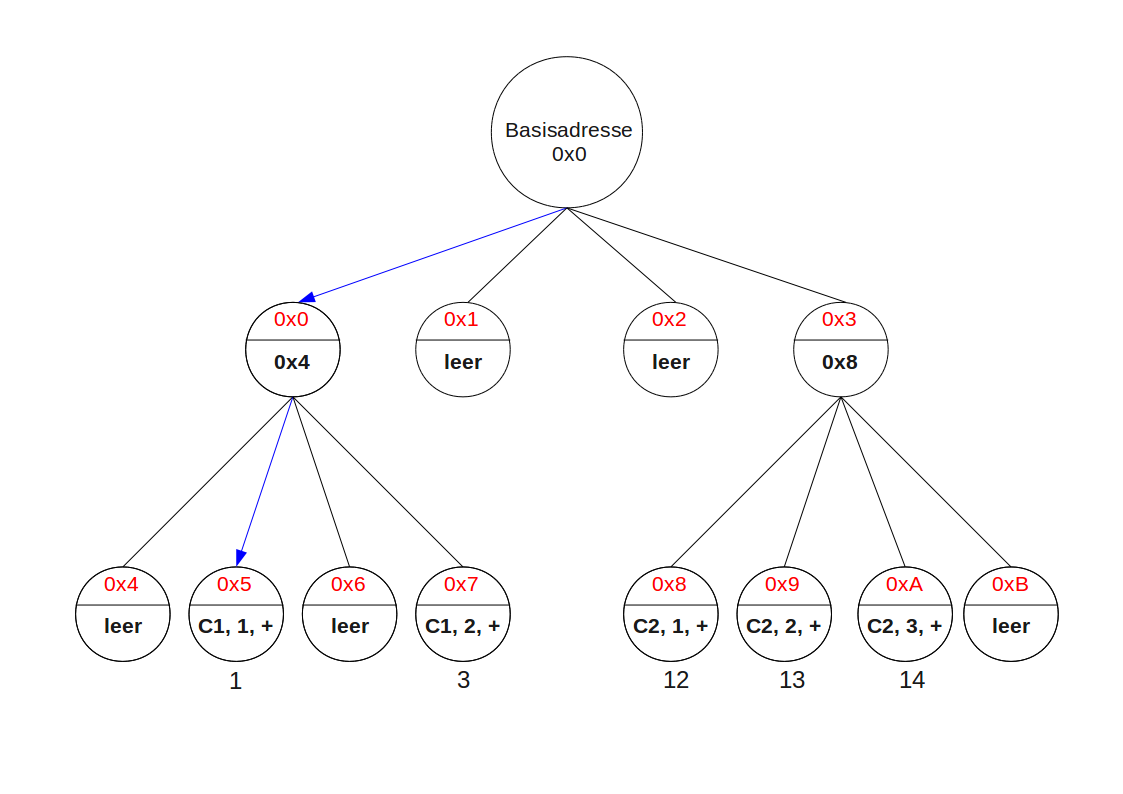
\includegraphics[width=\textwidth]{abb/tree.png}
  \caption{Baumstrukturierter Literal-Lookup}
  \label{tree}
\end{figure}
Mit einem Pfeil ist die Suche nach dem zugehörigen Tupel von 
Variable 1 markiert. Die Binärdarstellung von 1 ist 0001. Geteilt
in zwei Teile ergibt sich $t_1 = 00$ und $t_2 = 01$. Die Basisadresse 0x0 mit dem ersten
Teil $t_1$ addiert 0x0 + 00 ergibt 0x0. An Adresse 0x0 befindet sich die neue
Basisadresse 0x4. Nun addiert man den zweiten Teil $t_2$ mit der neuen Basisadresse
0x4 + 01 was 0x5 ergibt. An Adresse 0x5 findet man nun die Information, dass die Variable positiv ist und 
sich in der ersten Klausel C1 an der ersten Position befindet.\\
Zählt man nun die Knoten des Baumes in Abbildung \ref{tree}, stellt man fest, dass man 12 Knoten 
braucht, um diesen Baum aufzubauen. In Tabelle \ref{tree_table} ist der
Baum aus Abbildung \ref{tree} im Speicher eines Block-RAMs dargestellt.
\begin{table}[h]
  \centering
  \begin{tabular}{|l|l|l|}
    \hline
    \textsc{Speicheradresse} & \textsc{Daten}\\
    \hline
    0x0 & 0x4\\
    \hline
    0x1 & leer\\
    \hline
    0x2 & leer\\
    \hline
    0x3 & 0x8\\
    \hline
    0x4 & leer\\
    \hline
    0x5 & C1, 1, +\\
    \hline
    0x6 & leer\\
    \hline
    0x7 & C1, 2, +\\
    \hline
    0x8 & C2, 1, +\\
    \hline
    0x9 & C2, 2, +\\
    \hline
    0xA & C2, 3, +\\
    \hline
    0xB & leer\\
    \hline
    ... & ...\\
    \hline
  \end{tabular}
  \caption{Darstellung des Baumes aus Abbildung \ref{tree} im Speicher}
  \label{tree_table}
\end{table}
Man könnte sogar noch weitere Variablen 
hinzufügen, ohne weitere Knoten anlegen zu müssen (Wertetupel von 2 und 15).
Man kann also mit diesem Baum 8 von 15 Variablen referenzieren.
Allerdings kann man diese 8 Variablen nicht beliebig wählen.
Würde man zum Beispiel versuchen, Variable 4 in den Baum einzufügen müsste man 
den Knoten mit Adresse 0x1 expandieren, was eine Belegung von 4 weiteren 
Speicherplätzen mit sich führt.\\
Das Gruppieren von Formeln muss für diesen baumstruckturierten Literal-Lookup
weitere Bedingungen erfüllen. Hierfür werden folgende Begriffe eingeführt.

\begin{definition}
  Ein Baum $T$ ist ein Baum mit den folgenden Eigenschaften.
  \begin{itemize}
    \item Blätter sind entweder Tupel der Form (CID, POS, POL) oder leer
    \item Jeder nicht Blattknoten hat $2^m$ Kindsknoten und beinhaltet\\
      eine Basisadresse
    \item Die maximale Tiefe des Baumes ist $k/m$
  \end{itemize}
\end{definition}

\begin{function}
  Eine Funktion $tree(G)$ bildet einen Baum $T$ der Gruppe $G$.
\end{function}
\begin{function}
  Eine Funktion $mem(T)$ zählt die Knoten des Baumes $T$
\end{function}
mem(T) ermittelt somit den verbrauchten Speicherplatz. Mit $M$ wird
der verfügbare Speicherplatz bezeichnet.
\begin{function}
  Eine Funktion $add(v, T)$ fügt die Variable $v$ dem Baum $T$ hinzu.
\end{function}
\begin{function}
  Eine Funktion $add(C, T)$ fügt alle Literale $l_i \in C$
  dem Baum $T$ hinzu, indem iterativ die entsprechenden Variablen $v_i = var(l_i)$
  mit $add(v_i, T)$ dem Baum hinzugefügt werden.
\end{function}
Zu den Eigenschaften der Funktion $group: {\cal C} \rightarrow {\cal G}^{(1)}$
kommt nun noch eine weitere Bedingung, ob eine Klausel $C$ einer Gruppe $G_k \in {\cal G}^{(1)}$
hinzugefügt werden kann. Sollte die Relation $mem(add(C, tree(G_k))) \leq M$ erfüllt sein,
dann kann $C$ der Gruppe $G_k$ hinzugefügt werden.
Der Nachteil dieser vorgestellten Technik ist, dass sich der vorhandene Speicher 
für die Variablentupel mit einem Baum geteilt werden muss. Der geteilte Speicher hat zur
Folge, dass weniger Klauseln pro Gruppe möglich sind und somit
auch die Gesamtzahl der möglichen Klauseln sinkt. Es ist jedoch
auch möglich mehr Block-RAM für den Literal-Lookup zur Verfügung
zu stellen. Dann würde sich die Gesamtzahl möglicher Klauseln
nicht vermindern. Mehr Block-Ram ist auf größeren FPGAs
vorhanden, wie sie zum Beispiel von Davis \cite{davis:2008} benutzt werden.
Die Suche nach einem Variabletupel im Baum benötigt mehr Takte
als ein einfacher Speicherzugriff in der Literal-Lookup-Tabelle.
Da der Baum maximal $k/m$ Knoten tief ist, werden 
$k/m$ mal so viele Takte benötigt um ein Wertetupel zu finden.\\
Vorstellbar ist ein Baum mit k = 16 und m = 4. So könnte man 
Probleme mit $2^{16}$ Variablen lösen.

\subsection{Verbesserte Kommunikation zwischen FPGA und \\Host-PC}
\label{kommu}
Eine weitere Möglichkeit die Laufzeit des FPGA-Solvers zu
verbessern, ist es die Kommunikationzeit zwischen
Host-PC und FPGA zu minimieren. Eine Ethernetschnittstelle
ist zwar relativ einfach in Hardware zu implementieren,
jedoch hat sie höhere Latenzen als andere Kommunukationsschnittstellen wie
PCI Express \cite{pcie:2006} oder Hyper-Transport \cite{ht:2006}.
In einem Vergleich \cite{htvspcie:2006} der Latenzen von PCI-E und HT
wurden Übertragungszeiten der beiden Schnittstellen gemessen.
Die Zeiten liegen weit unter der Latenz eines Ethernet-Pakets (300 $\mu$s)
bei ca. 1 $\mu$s.\\
An einigen Stellen im Entwurf ist es nicht unbedingt notwendig,
dass der FPGA auf Antwortpakete des Host-PCs wartet. Angenommen
der FPGA speichert sich die Information ob ein Literal ein Entscheidungsliteral
ist. Im Konfliktfall informiert der FPGA zwar den Host
über die aktuelle Situation, kann dann jedoch den Konflikt
selbst auflösen. Dies würde eine Verschränkung der Kommunikation
zwischen FPGA und Host-PC bedeuten und Kommunikationszeit
einsparen.


\subsection{Conflict Driven Clause Learning Algorithmus}
\label{cdcl}
In diesem Abschnitt soll die Verwendung von CDCL als
Suchalgorithmus zum Lösen von  SAT-Problemen untersucht werden.
Der Conflict Driven Clause Learning Algorithmus (CDCL) ist eine
Erweiterung des \\DPLL-Algorithmus und wurde in \cite{paper:silva:1997} eingeführt.
Der CDCL-Algorithmus versucht aus Konflikten zu lernen. Bei einem Konflikt wird die
entsprechende Konfliktklausel (unerfüllte Klausel, welche einen Konflikt auslöst)
analysiert, eine neue Klausel gelernt und ein Rücksprung über
mehrere Entscheidungsliterale hinweg duchgeführt.\\
Den massiven Geschwindigkeitsgewinn, gegenüber DPLL-Solvern,  
hat ein CDCL-Solver einer vielzahl von eingesetzten Techniken 
zu verdanken.
In der Arbeit von Katebi \cite{katebi:2011} wird untersucht,
welchen Einfluss einzelne Techniken auf das Zeitverhalten
von SAT-Solvern haben. Dabei werden sowohl DPLL- als auch 
CDCL-Solver betrachtet. Folgende Techniken wurden untersucht:\\
\begin{itemize}
\item 
  Two Literal Watching (2WL) \cite{moskewicz:2001}
\item 
  Phase Saving (PHS) \cite{pipatsrisawar:2007}
\item 
  Random Restarts (RST) \cite{gomes:1998}
\item 
  Variable State Independent Decaying Sum (VSIDS) \cite{moskewicz:2001}
\item 
  Clause Learning (CL) \cite{paper:silva:1997}
\end{itemize}
\begin{figure}[h]
  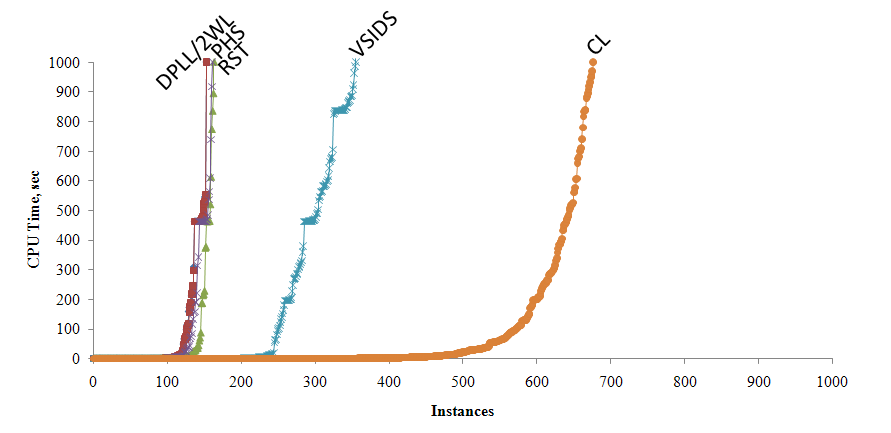
\includegraphics[width=\textwidth]{abb/dpll-teq.png}
  \caption{DPLL-Techniken  \cite{katebi:2011}}
  \label{dpll-teq}
\end{figure}
In Abbildung \ref{dpll-teq} sind die Ergebnisse der Untersuchungen von Katebi, über 1000 SAT-Instanzen,
dargestellt. Beim lösen der Instanzen gibt es ein Zeitlimit von 1000 Sekunden. Man sieht wieviele Instanzen 
der DPLL-Solver durch hinzunahme verschiedener
Techniken lösen kann. Die wenigsten Instanzen löst der reine DPLL-Solver. Auch 
das Erweitern des Solvers durch 2WL, PHS, oder RST ermöglicht es nicht wesentlich
mehr Instanzen zu lösen. Die Techniken VSIDS und CL sorgen für einen starken
Leistungsschub. Wobei sich VSIDS leicht auf dem Host-PC des FPGA-Solvers implementieren
lässt, da es sich um eine Entscheidungsheuristik handelt. Der FPGA müsste dem Host-PC
nur noch die Konfliktklausel mitteilen, da diese für die Berechnung des nächsten
Entscheidungsliterals eine wichtige Rolle spielt. Um CL ohne weiteres implementieren
zu können, müsste es dem FPGA-Solver möglich sein weitere Klauseln zu lernen und
somit seine Klauseldatenbank zu aktualisieren.
Das lernen von Klausel ist jedoch im aktuellen Entwurf nicht vorgesehen. Im
Entwurf von Davis wird eine Technik beschrieben, so dass auch ein FPGA-Solver
Klauseln lernen kann.\\
Abbildung \ref{cdcl-teq} zeigt zusätzlich noch Ergebnisse eines CDCL-Solvers. Es wurden die gleichen 
Instanzen gelöst wie auch in Abbildung \ref{dpll-teq}. Der genutzte CDCL-Solver implementiert alle
oben aufgeführten Techniken. Der Graph, welcher mit $\neg$ CL
beschriftet ist, zeigt die Ergebnisse eines CDCL-Solvers ohne
Clause Learning.
\begin{figure}[h]
  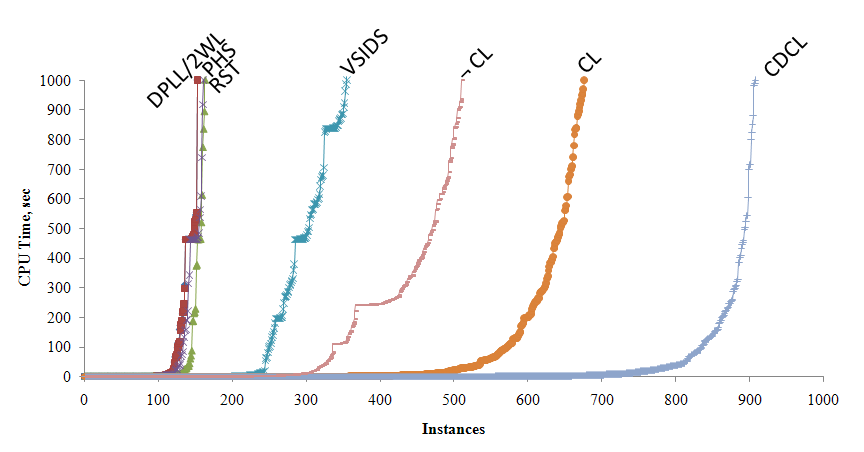
\includegraphics[width=\textwidth]{abb/cdcl-teq.png}
  \caption{CDCL-Techniken \cite{katebi:2011}}
  \label{cdcl-teq}
\end{figure}
Man sieht, das ein CDCL-Solver ohne CL mehr Instanzen löst als
ein DPLL-Solver erweitert mit VSIDS. Es ist also möglich den Algorithmus
des Host-PCs auf CDCL ohne CL umzustellen ohne große Veränderungen
am Entwurf des FPGAs vorzunehmen und trotzdem einen
Leistungsgewinn zu erhalten.





\bibliography{mybib}

\end{document}
%%% DOKUMENT ENDE %%%%%%%%%%%%%%%%%%%%%%%%%%%%%%%%%%%%%
%%%%%%%%%%%%%%%%%%%%%%%%%%%%%%%%%%%%%%%%%%%%%%%%%%%%%%%
